% =====================================================================
% Bachelorarbeit — HSW FHNW. Angepasst an FHNW-Vorgaben (APA 7 dt.,
% Pflichtstruktur). Kompiliert mit pdfLaTeX + Biber.
% Vorgaben dokumentiert in docs/project/FHNW_VORGABEN.md.
% Schweizer Orthografie: ss statt scharfem s.
% =====================================================================
\documentclass[11pt,a4paper]{report}

\usepackage[utf8]{inputenc}
\usepackage[T1]{fontenc}
\usepackage{lmodern}
\usepackage[ngerman]{babel}
\usepackage[a4paper,left=3cm,right=2.5cm,top=2.5cm,bottom=2.5cm]{geometry}
\usepackage{setspace}
\onehalfspacing
\usepackage{graphicx}
\graphicspath{{figures/}}
\usepackage{booktabs}
\usepackage{microtype}

% --- Zitierstil: APA (deutsch) via apacite, natbibapa-Modus ---
% apacite ist bibtex-basiert (kompiliert zuverlässig auf Overleaf-Gratisplan).
% natbibapa lädt natbib: bestehende \citep/\citet funktionieren weiter.
\usepackage[natbibapa]{apacite}
\usepackage[hidelinks]{hyperref}
\AtBeginDocument{\renewcommand{\bibname}{Literaturverzeichnis}}

\begin{document}

% ====================== Titelseite ======================
\begin{titlepage}
\centering
{\large Fachhochschule Nordwestschweiz FHNW\\
Hochschule für Wirtschaft\par}
\vspace{0.3cm}
{\large Bachelor of Science FHNW in Business Artificial Intelligence\par}% Studiengang prüfen
\vspace{2.2cm}
{\large Bachelor Thesis\par}
\vspace{1.2cm}
{\huge\bfseries Informationelle Effizienz dezentraler Prognosemärkte\par}
\vspace{0.5cm}
{\Large am Beispiel Polymarket im Vergleich zu traditionellen Prognosequellen\par}
\vspace{2.5cm}
\begin{tabular}{rl}
Verfasser: & Pablo Cruz\\[2pt]
Matrikelnummer: & [Matrikelnummer einfügen]\\[2pt]
Betreuende Person: & [Dozent/in einfügen]\\[2pt]
Auftraggeberschaft: & Neutralnews\\[2pt]
Standort: & [Basel/Brugg/Olten]\\[2pt]
Abgabedatum: & [TT.MM.2026]\\
\end{tabular}
\vfill
\end{titlepage}

\pagenumbering{roman}
\setcounter{page}{2}

% ====================== Eigenständigkeitserklärung ======================
\chapter*{Eigenständigkeitserklärung}
Ich erkläre hiermit, dass ich die vorliegende Bachelor Thesis selbständig und
ohne Benutzung anderer als der angegebenen Quellen und Hilfsmittel verfasst habe.
Alle Stellen, die wörtlich oder sinngemäss aus Quellen entnommen wurden, sind als
solche kenntlich gemacht und im Literaturverzeichnis aufgeführt. Sämtliche bei der
Erstellung dieser Arbeit verwendeten Hilfsmittel --- insbesondere Lektorate und
KI-Tools --- sind im Hilfsmittelverzeichnis vollständig deklariert.

\vspace{1.5cm}
\noindent Ort, Datum: \rule{5cm}{0.4pt} \hfill Unterschrift: \rule{5cm}{0.4pt}

% ====================== Hilfsmittelverzeichnis ======================
\chapter*{Hilfsmittelverzeichnis}
\addcontentsline{toc}{chapter}{Hilfsmittelverzeichnis}
Folgende Hilfsmittel wurden bei der Erstellung dieser Arbeit eingesetzt. Massgebend
ist das Merkblatt ``Einsatz von KI-Tools'' der HSW FHNW. Alle inhaltlichen Aussagen
wurden von der Verfasserin/dem Verfasser geprüft und verantwortet.

\begin{itemize}
  \item \textbf{KI-Tools:} [z.B. ChatGPT, Claude] --- eingesetzt für [z.B.
  Strukturierung, Recherche-Unterstützung, Code-Hilfe, sprachliche Überarbeitung].
  Keine Übernahme unüberprüfter Inhalte.
  \item \textbf{Statistik/Code:} Python (pandas, numpy, scipy, statsmodels,
  matplotlib), SQLite, DuckDB --- sämtliche statistischen Kennzahlen wurden
  deterministisch berechnet und getestet.
  \item \textbf{Literaturverwaltung:} Zotero mit Better BibTeX.
  \item \textbf{Lektorat:} [falls zutreffend: Person/Tool].
\end{itemize}

% ====================== Management Summary ======================
\chapter*{Management Summary}
\addcontentsline{toc}{chapter}{Management Summary}
% Entwurf — vor Abgabe verdichten. Das öffentliche Management Summary
% (Moodle-Formular, 300/600/600/1200 Zeichen) ist separat.
\textbf{Ausgangslage.} Dezentrale Prognosemärkte wie Polymarket bündeln
verteiltes Wissen zu Wahrscheinlichkeiten und standen während der US-Wahl 2024 in
Spannung zu traditionellen Umfragen. Die Arbeit untersucht, wie effizient
Polymarket Information verarbeitet.

\textbf{Vorgehen.} Informationelle Effizienz wird über drei deterministisch in
Python berechnete Proxy-Hypothesen geprüft: Prognosequalität (Brier/Diebold-Mariano,
H1), tägliche Ereignisreaktion (H2) und Wallet-Tier-Timing (Granger, H3), ergänzt
um einen read-only Anomalie-Monitor und eine Schweizer Referendums-Fallstudie.

\textbf{Ergebnisse.} Polymarket zeigt in einem klar abgegrenzten Vergleichsfenster
bessere Prognosequalität (262 von 285 State-Date-Zeilen), aber keine universelle
Überlegenheit, die Tagesreaktion auf kuratierte Ereignisse ist plausibel, das
oberste Wallet-Tier zeigt das klarste prädiktive Timing-Muster. Die Befunde
stützen begrenzte, reproduzierbare Diagnosen, keine pauschale Effizienz- oder
Handelsaussage.

% ====================== Verzeichnisse ======================
\tableofcontents
\clearpage
\listoffigures
\addcontentsline{toc}{chapter}{Abbildungsverzeichnis}
\listoftables
\addcontentsline{toc}{chapter}{Tabellenverzeichnis}

% ====================== Hauptteil ======================
\clearpage
\pagenumbering{arabic}
% Status: ueberarbeitet nach FHNW-Struktur fuer empirische Arbeiten
% (docs/project/FHNW_ACADEMICGUIDE_RULES.md, Abschnitt 4a + 10).
% Evidence: method_h1_brier_dm; method_h2_event_window; method_h3_wallet_tiers.
% Finale Zitation nach Quellenreview (docs/project/SOURCE_REVIEW_LOG.md).
\chapter{Einleitung}
\label{ch:intro}

\section{Ausgangslage und Problemstellung}
Prognosemaerkte buendeln das verteilte Wissen vieler Marktteilnehmender in einem
einzigen, laufend aktualisierten Preis, der sich als Wahrscheinlichkeit fuer ein
kuenftiges Ereignis lesen laesst. Die theoretische Grundlage bildet die
Markteffizienzhypothese, nach der Preise die verfuegbare Information widerspiegeln
\citep{lit_emh_001}. Im US-Wahljahr 2024 wurde der dezentrale, auf der Blockchain
abgewickelte Markt Polymarket zum sichtbarsten Beispiel dieser Idee. Er erreichte
zeitweise sehr hohe Handelsvolumina und stand wiederholt in Spannung zu
traditionellen Umfragen und Forecast-Modellen, die ein knapperes Rennen zeichneten
\citep{zotero_poly_001,zotero_poly_009}.

Diese Diskrepanz wirft eine grundlegende Frage auf. Verarbeitet ein solcher Markt
Information tatsaechlich besser als etablierte Quellen, oder erscheint er nur
deshalb ueberlegen, weil einzelne Episoden im Nachhinein betont werden? Die
vorliegende Arbeit nimmt diese Frage zum Ausgangspunkt und untersucht die
informationelle Effizienz von Polymarket im Kontext der US-Praesidentschaftswahl
2024 --- nicht als pauschale Behauptung, sondern als nachvollziehbar gepruefte,
scope-spezifische Aussage.

\section{Relevanz und Einordnung}
Die Fragestellung ist wirtschaftlich wie methodisch relevant. Erstens ruecken
Prognosemaerkte als kostenguenstige, laufend aktualisierte Forecast-Infrastruktur
in den Blick von Unternehmen, Medien und oeffentlichen Institutionen, die auf
verlaessliche Wahrscheinlichkeitsschaetzungen angewiesen sind. Zweitens macht die
Blockchain-Abwicklung jede Transaktion oeffentlich nachvollziehbar und eroeffnet
damit Analysen auf Wallet-Ebene, die in traditionellen Maerkten nicht moeglich
sind \citep{zotero_poly_001}. Drittens beruehrt die Diskussion um Grosskonten und
moeglichen informierten Handel Fragen der Marktintegritaet und der Regulierung
\citep{zotero_poly_005,zotero_poly_007}.

Eine reproduzierbare und methodisch vorsichtige Untersuchung leistet damit einen
doppelten Beitrag. Sie ordnet die empirische Effizienzforschung zu dezentralen
Maerkten ein und liefert zugleich eine praxisnahe Grundlage, um die Verlaesslichkeit
solcher Maerkte realistisch und ohne ueberzogene Erwartungen einzuschaetzen.

\section{Forschungsfrage und Hypothesen}
Aus der Problemstellung leitet sich die folgende Forschungsfrage ab:

\begin{quote}
In welchem Mass verarbeitet Polymarket waehrend der US-Praesidentschaftswahl 2024
Information, verglichen mit traditionellen Prognosequellen?
\end{quote}

Informationelle Effizienz \citep{lit_emh_001} wird dabei nicht direkt behauptet,
sondern ueber drei reproduzierbare, deterministisch pruefbare Proxy-Hypothesen
operationalisiert:

\begin{itemize}
  \item \textbf{H1 (Prognosequalitaet):} Polymarket liefert besser oder gleich gut
  kalibrierte Wahrscheinlichkeiten wie vergleichbare traditionelle Forecasts,
  gemessen am Brier-Verlust \citep{lit_brier_001} und am
  Diebold-Mariano-Vergleich der Verlustreihen \citep{lit_dm_001}.
  \item \textbf{H2 (Ereignisreaktion):} Die Polymarket-Wahrscheinlichkeiten bewegen
  sich um vorab kuratierte oeffentliche Ereignisse in plausibler Richtung,
  untersucht mit einem Ereignisstudien-Design \citep{lit_eventstudy_001}.
  \item \textbf{H3 (Wallet-Timing):} Dataset-relative Wallet-Tiers zeigen zeitliche
  Aktivitaetsmuster um Preisbewegungen, gemessen ueber Lead-Lag-Korrelationen und
  Granger-Tests \citep{lit_granger_001}.
\end{itemize}

Die drei Hypothesen greifen ineinander. H1 prueft die Ergebnisqualitaet der
Prognose, H2 die Reaktionsrichtung auf neue oeffentliche Information und H3 die
zeitliche Struktur der zugrunde liegenden Handelsaktivitaet. Zusammen erlauben sie
eine differenzierte statt einer pauschalen Antwort auf die Forschungsfrage.

\section{Abgrenzung des Untersuchungsgegenstands}
Der Untersuchungsgegenstand ist bewusst eng gefasst. Untersucht wird die US-Wahl
2024 als einzelner Fallkontext, Polymarket bildet die primaere Zeitreihe,
traditionelle Umfragen und Modell-Forecasts dienen als Vergleich. Die Arbeit erhebt
ausdruecklich keinen Anspruch auf universelle Markteffizienz, auf
Intraday-Reaktionsgeschwindigkeit, auf kausale Insider-Effekte oder auf handelbare
Profitabilitaet. Die Wallet-Analyse stuetzt sich auf oeffentliche, quellseitig
gefilterte Kauf-Transaktionen und ist deshalb als deskriptive Timing-Diagnostik zu
lesen, nicht als Nachweis privater Information.

Diese Selbstbeschraenkung folgt der in der Literatur betonten Vorsicht. Grosskonto-
Aktivitaet kann mit heterogenen Erwartungen statt mit Manipulation vereinbar sein
\citep{zotero_poly_001}, und Prognosemaerkte koennen reflexive Verzerrungen
aufweisen, die ihre Genauigkeit begrenzen \citep{zotero_poly_009}.

\section{Forschungsluecke und Beitrag}
Die bestehende Literatur liefert Theorie zur Informationsaggregation, etablierte
Messverfahren und gemischte Evidenz zu Polymarket, behandelt diese Aspekte aber
meist getrennt \citep{zotero_poly_002,zotero_poly_007}. Was fehlt, ist eine
reproduzierbare, deterministisch gepruefte Zusammenfuehrung von Prognosequalitaet,
Ereignisreaktion und On-Chain-Timing fuer denselben Marktkontext. Genau diese Luecke
schliesst die Arbeit fuer die US-Wahl 2024.

Der empirische Kern ist ein vollstaendig deterministischer, getesteter
Python-Analysepfad, der alle Kennzahlen berechnet, bevor sie interpretiert werden.
Als Sekundaerbeitraege dokumentiert die Arbeit ein aus der Untersuchung
hervorgegangenes read-only Monitoring-Werkzeug sowie die Multiagenten-Methodik
seiner Entwicklung (Kapitel~\ref{ch:erweiterungen}). Diese Sekundaerbeitraege
stuetzen die Forschungsfrage, ersetzen aber den empirischen Beleg nicht und
ueberlagern ihn nicht.

\section{Aufbau der Arbeit}
Die Arbeit ist in der Struktur einer empirischen Forschungsarbeit aufgebaut.
Kapitel~\ref{ch:theorie} ordnet Theorie und Literatur ein und entwickelt die
Forschungsluecke. Kapitel~\ref{ch:methodik} beschreibt Daten, Aufbereitung und die
deterministischen Verfahren fuer H1 bis H3. Die Kapitel~\ref{ch:h1} bis
\ref{ch:h3} berichten die Ergebnisse der drei Hypothesen. Kapitel~\ref{ch:erweiterungen}
stellt die Erweiterungen vor, darunter den Monitor, die Schweizer Fallstudie und
den praktischen Beitrag. Kapitel~\ref{ch:diskussion} fuehrt die Befunde zusammen,
diskutiert die Limitationen und zieht das Fazit, und Kapitel~\ref{ch:ausblick}
skizziert den agentengestuetzten Ausblick.

% Status: überarbeitet als FHNW-Literatur-Review (Begriffe, Theorie, Best
% Practice, Vorbefunde, Forschungslücke). Strukturvorlage angepasst an die
% eigene Arbeit (docs/project/FHNW_ACADEMICGUIDE_RULES.md, Abschnitt 4 + 10).
% Finale Zitation nach Quellenreview (docs/project/SOURCE_REVIEW_LOG.md).
\chapter{Theoretischer Rahmen und Forschungsstand}
\label{ch:theorie}

Dieses Kapitel ordnet die für die Arbeit relevanten Begriffe, Theorien,
Messverfahren und Vorbefunde ein. Es folgt der Logik eines Literatur-Reviews.
Zuerst werden die zentralen Begriffe geklärt, danach die theoretischen
Grundlagen und die etablierten Verfahren zur Messung von Prognosequalität und
Marktreaktion dargestellt, anschliessend die bisherige Forschung zu Polymarket
und zu informiertem Handel diskutiert. Aus dieser Zusammenschau ergibt sich die
Forschungslücke, welche die drei Hypothesen motiviert. Ausgewählt werden nur
jene Konzepte und Quellen, die für die Forschungsfrage unmittelbar relevant sind.

\section{Begriffsklärung}
Ein \emph{Prognosemarkt} ist ein Markt, auf dem Kontrakte auf den Ausgang
künftiger Ereignisse gehandelt werden und dessen Preis sich als kollektive
Wahrscheinlichkeitsschätzung lesen lässt \citep{zotero_poly_005}. Ein binärer
Kontrakt zahlt bei Eintritt des Ereignisses einen festen Betrag und sonst nichts,
sodass der Gleichgewichtspreis zwischen null und eins der vom Markt
eingepreisten Eintrittswahrscheinlichkeit entspricht. \emph{Informationelle
Effizienz} bezeichnet den Grad, in dem dieser Preis die öffentlich verfügbare
Information widerspiegelt \citep{lit_emh_001}. Die Arbeit verwendet den Begriff
bewusst graduell und scope-spezifisch, nicht als absolute Eigenschaft.

\emph{Kalibrierung} meint die Uebereinstimmung von prognostizierter
Wahrscheinlichkeit und beobachteter relativer Häufigkeit: Ereignisse, denen ein
Markt 70 Prozent zuweist, sollten langfristig in etwa 70 Prozent der Fälle
eintreten. \emph{Polymarket} ist ein dezentraler, auf einer Blockchain
abgewickelter Prognosemarkt, bei dem jede Transaktion öffentlich einsehbar ist.
Eine \emph{Wallet} ist die öffentliche Adresse, über die eine Teilnehmerin oder
ein Teilnehmer handelt. Ein \emph{Tier} ist in dieser Arbeit eine
dataset-relative Grössenklasse von Wallets, abgeleitet aus den beobachteten
kumulierten Betragsperzentilen und nicht aus einer willkürlichen
Dollar-Schwelle. Diese Begriffe bilden die gemeinsame Grundlage der drei
Hypothesen.

\section{Markteffizienz und Informationsaggregation}
Der theoretische Ausgangspunkt ist die Markteffizienzhypothese
\citep{lit_emh_001}, nach der Preise verfügbare Information widerspiegeln. Ueblich
ist die Unterscheidung in eine schwache, eine halbstrenge und eine strenge Form,
je nachdem, ob historische Preise, alle öffentlichen Informationen oder auch
private Informationen bereits eingepreist sind. Auf Prognosemärkte übertragen
heisst das: Wenn genügend Teilnehmende ihre Erwartungen laufend an neue Evidenz
anpassen, sollte der Marktpreis als Wahrscheinlichkeit die verfügbare
Information bündeln.

Diesen Aggregationsmechanismus beschreibt \citet{zotero_poly_005} konzeptionell
und verweist auf Vergleiche, in denen spekulative Märkte Experteneinschätzungen
und Umfragen erreichen oder schlagen. Die Idee der Informationsaggregation
(häufig als Weisheit der Vielen bezeichnet) motiviert überhaupt erst, einen
Marktpreis als Forecast zu behandeln. Sie ist zugleich eine Annahme, die
empirisch zu prüfen und nicht vorauszusetzen ist.

\section{Prognosemärkte im Vergleich zu traditionellen Quellen}
Ob Märkte Umfragen tatsächlich überlegen sind, ist empirisch umstritten.
\citet{zotero_poly_002} finden für die US-Wahl 2024 einen Vorteil von Polymarket
gegenüber Umfragen, besonders in den umkämpften Swing States, und ordnen ihn der
Wisdom-of-Crowds-Idee zu. Zugleich betonen sie ausdrücklich, dass die Ergebnisse
weiterer Untersuchung und einer Prüfung auf Uebertragbarkeit bedürfen. Dem steht
eine kritische Sicht gegenüber: \citet{zotero_poly_009} argumentiert, dass
Prognosemärkte keine "Truth Machine" sind, sondern reflexiv sein können ---
Vertrauen in den Marktpreis kann die laufende Informationsaktualisierung
schwächen und so die Genauigkeit untergraben.

Auch die Mikrostruktur solcher Märkte ist relevant. \citet{zotero_poly_006}
analysieren am Beispiel von Kalshi das Zusammenspiel von liquiditätsgebenden und
liquiditätsnehmenden Teilnehmenden und zeigen, dass die Preisqualität von der
Marktstruktur und den Anreizen abhängt. Diese Spannung zwischen belegtem Vorteil
und berechtigter Vorsicht begründet, warum die vorliegende Arbeit nur begrenzte,
scope-spezifische Aussagen anstrebt.

\section{Messung von Prognosequalität}
Zur Messung der Forecast-Qualität dient der Brier-Score \citep{lit_brier_001},
definiert als mittlere quadratische Abweichung zwischen Wahrscheinlichkeitsprognose
und tatsächlichem Ausgang. Ein niedrigerer Brier-Verlust bedeutet eine bessere
Prognose, und der Score belohnt sowohl Treffsicherheit als auch gute Kalibrierung.
Der Vergleich zweier Verlustreihen erfolgt mit dem Diebold-Mariano-Test
\citep{lit_dm_001}, der prüft, ob zwei Prognosen im Mittel gleich genau sind, ohne
einen bestimmten Entstehungsmechanismus zu unterstellen. Beide Verfahren gelten
als etablierte, deterministisch berechenbare Masse der Forecast-Bewertung und
bilden die methodische Grundlage von H1.

\section{Ereignisstudien}
Die Reaktion eines Marktes auf neue Information lässt sich mit Ereignisstudien
untersuchen \citep{lit_eventstudy_001}. Das Verfahren definiert ein Schätzfenster
für das normale Verhalten und ein Ereignisfenster, in dem abnormale und
kumulierte abnormale Bewegungen gemessen werden. Ursprünglich für Aktienrenditen
entwickelt, lässt sich das Design auf Tagesebene und auf Wahrscheinlichkeits-
zeitreihen übertragen. H2 nutzt dieses Design mit vorab fixierten, kuratierten
öffentlichen Ereignissen, um die Reaktionsrichtung von Polymarket nachvollziehbar
zu prüfen.

\section{On-Chain-Aktivität und informierter Handel}
Die Blockchain-Abwicklung macht Wallet-Aktivität sichtbar und eröffnet die Frage,
ob bestimmte Adressen Preisbewegungen zeitlich vorauslaufen. Methodisch nutzt H3
Lead-Lag-Korrelationen und Granger-Tests \citep{lit_granger_001}, deren Ergebnisse
ausdrücklich als prädiktive Timing-Diagnostik und nicht als strukturelle
Kausalität zu lesen sind. Theoretisch rahmt das Modell von \citet{lit_kyle_001}
informierten Handel: Eine informierte Partei verbirgt ihre Order im normalen
Handelsfluss, was sich in abnormaler Handelsgrösse niederschlagen kann. Empirisch
zeigt \citet{zotero_delvecchio_001} für Kalshi-Märkte, dass informierter Handel
real und über eine Abnormal-Trade-Size-Kennzahl detektierbar ist und sich gegen
die Marktauflösung verstärkt.

Für die gebotene Vorsicht sprechen mehrere Befunde. \citet{zotero_poly_001} zeigen
für die Oktober-Grosskonto-Episode 2024, dass Kapital gleichzeitig auf beide
Marktseiten floss --- ein Muster, das mit heterogenen Erwartungen und nicht mit
einseitiger Manipulation vereinbar ist. \citet{zotero_poly_007} ergänzt
Verhaltensverzerrungen, etwa die Ueberschätzung kleiner Wahrscheinlichkeiten,
sowie eine im Vergleich zu traditionellen Instrumenten höhere Volatilität. In der
Praxis setzt Polymarket inzwischen eine On-Chain-Ueberwachung ein, die unter
anderem ungewöhnliche Positionsgrössen vor Ergebnissen flaggt
\citep{news_polymarket_integrity_001}, gestützt auf forensische Heuristiken wie
Funding-Quellen und Wallet-Clustering \citep{news_chainalysis_forensics_001}.
Diese Arbeiten liefern gemeinsam eine Signatur informierten Handels, ohne dass
einzelne Adressen damit als Insider bewiesen wären.

\section{Forschungslücke}
Die Literatur liefert Theorie zur Aggregation und Effizienz, etablierte Methodik
(Brier, Diebold-Mariano, Ereignisstudien, Granger) und gemischte Evidenz zu
Polymarket. Diese Bausteine werden jedoch meist getrennt behandelt: Prognosequalität,
Ereignisreaktion und On-Chain-Timing erscheinen in unterschiedlichen Arbeiten und
selten für denselben Marktkontext. Was fehlt, ist eine reproduzierbare,
deterministisch geprüfte Zusammenführung dieser drei Perspektiven für einen
gemeinsamen Fall. Genau diese Lücke schliesst die vorliegende Arbeit für die
US-Wahl 2024, indem sie H1, H2 und H3 auf derselben Datenbasis und mit
nachvollziehbaren, vorab festgelegten Verfahren untersucht.

% Status: bounded-draft-ready. Inhaltlich vollständig, finale Zitation
% nach Quellenreview. Quelle: docs/research/THESIS_KAPITEL_03_METHODIK_DRAFT.md
\section{Daten und Methodik}
\label{ch:methodik}

\subsection{Forschungsdesign: deterministischer Kern vor Interpretation}

Die Arbeit prüft informationelle Effizienz nicht als direkt beobachtbare
Eigenschaft, sondern über drei reproduzierbare Proxy-Tests: Prognosequalität
(H1), Ereignisreaktion (H2) und Wallet-Timing (H3). Diese Operationalisierung
folgt dem Effizienzbegriff der Markteffizienzhypothese \citep{lit_emh_001} und
überträgt ihn auf einen dezentralen Prognosemarkt, dessen Preispfad als
primäre Zeitreihe behandelt wird.

Methodisch gilt eine strikte Trennung: Alle statistischen Kennzahlen werden
deterministisch in Python berechnet, versioniert und als Artefakt (CSV, JSON,
PNG) abgelegt. Sprachmodelle oder Agenten berechnen keine Metriken, sie dürfen
ausschliesslich bereits berechnete, begrenzte Ergebnisse interpretieren, und
auch das erst nach dokumentierter Freigabe und Audit-Protokollierung. Diese
Reihenfolge --- Datenvalidierung, deterministische Analyse, danach Interpretation
--- sichert Nachvollziehbarkeit und schützt vor versteckten Berechnungen im
Fliesstext.

\subsection{Datenbasis}

Die empirische Basis liegt in einer lokalen SQLite-Datenbank
(\texttt{data/thesis.db}). Tabelle~\ref{tab:t1} fasst Quellen, Zeilenzahlen und
bekannte Einschränkungen zusammen.

\begin{table}[ht]
\centering
\caption{Daten- und Quelleninventar (T1)}
\label{tab:t1}
\small
\begin{tabular}{@{}llll@{}}
\toprule
Quelle & Tabelle & Umfang & Rolle / Einschränkung \\
\midrule
Polymarket CLOB/Gamma & \texttt{polymarket\_prices} & 307 Tagespreise & primäre Marktzeitreihe \\
FiveThirtyEight & \texttt{poll\_forecasts} & 245 Zeilen & Vergleichsquelle H1 \\
On-Chain-Wallets & \texttt{whale\_trades} & 25\,113 Zeilen & H3, BUY-only, Filter $\geq$10\,000 USD \\
GDELT & \texttt{sentiment\_scores} & 310 Zeilen & Kontext, kein Kernparameter \\
Ereigniskatalog (Seed) & \texttt{events\_timeline} & 7 kuratierte Ereignisse & H2-Eingabe, vorab fixiert \\
\bottomrule
\end{tabular}
\end{table}

Die Vergleichsquellen sind bewusst restriktiv gewählt. FiveThirtyEight liefert
native Wahrscheinlichkeiten und ist deshalb direkt vergleichbar
\citep{zotero_poly_002}. Für die Kalibrierungsdiagnostik in H1 treten als weitere aufgelöste Vergleichsquellen das unabhängige Umfragemodell Rieke, die 270toWin/JHK-Staatenprognose sowie eine dokumentierte Umfrage-Transformation (Poll-Transform) hinzu, jeweils nur für den paarweisen Brier-Vergleich und nicht als Kernzeitreihe. RealClearPolitics liefert Umfragedurchschnitte, keine
Prognosewahrscheinlichkeiten, diese Quelle bleibt aus allen Wahrscheinlichkeits-
und Kalibrierungsmetriken ausgeschlossen, solange die in der Methodiknote
(\texttt{docs/research/RCP\_TRANSFORMATION.md}) beschriebene Logit-Transformation
nicht freigegeben ist. Die Wallet-Daten tragen die methodisch wichtigste
Datenlimitation: Sie enthalten nur Kauftransaktionen und sind quellseitig ab
10\,000 USD gefiltert, beides bleibt Metadaten-Eigenschaft der Rohquelle und ist
keine analytische Schwellendefinition.

\subsection{Operationalisierung der Hypothesen}

\paragraph{H1 --- Prognosequalität}
H1 bewertet, ob Polymarket im überlappenden Vergleichsfenster bessere
Prognosequalität zeigt als vergleichbare traditionelle
Wahrscheinlichkeitsprognosen. Als Verlustmass dient der Brier-Score
\citep{lit_brier_001}, der paarweise Vergleich der Verlustreihen erfolgt mit dem
Diebold-Mariano-Test \citep{lit_dm_001}, ergänzt um Kalibrierungsdiagnostik,
soweit Stichprobengrösse und Methodik es zulassen. Erlaubt ist ausschliesslich
die Aussage eines Prognosequalitäts-Vergleichs, ein Beweis höherer
Reaktionsgeschwindigkeit, eine allgemeine Marktüberlegenheit oder eine
RCP-Wahrscheinlichkeitsaussage ohne dokumentierte Transformation sind
ausgeschlossen.

\paragraph{H2 --- Ereignisfenster}
H2 prüft, ob sich Polymarket-Wahrscheinlichkeiten um vorab kuratierte
öffentliche Ereignisse in plausibler Richtung und innerhalb fester Tagesfenster
bewegen. Die Ereignisse werden vor der Analyse mit Zeitstempel, Quelle und
erwarteter Richtung fixiert und nach Sichtung der Marktreaktion weder
hinzugefügt noch entfernt. Das Design folgt der Ereignisstudien-Methodik
\citep{lit_eventstudy_001}. Erlaubt ist die Aussage einer täglichen
Ereignisfenster-Reaktion, ein Intraday-Geschwindigkeitsanspruch oder eine
nachträgliche Ereignisauswahl sind ausgeschlossen.

\paragraph{H3 --- Wallet-Timing}
H3 untersucht, ob dataset-relative Wallet-Tiers zeitliche Aktivitätsmuster vor
oder um Polymarket-Preisbewegungen zeigen. Die Tiers werden nicht über eine
willkürliche USD-Schwelle definiert, sondern aus den beobachteten kumulierten
Betragsperzentilen der Wallet-Verteilung abgeleitet. Die Diagnostik kombiniert
deskriptive Lead-Time-Histogramme, Lead-Lag-Korrelationen und Granger-Tests
\citep{lit_granger_001}. Die Granger-Ausgaben werden als prädiktive
Timing-Diagnostik unter Modellannahmen gelesen, nicht als Kausalitätsbeweis,
die Vorsicht gegenüber Insider-Interpretationen stützt sich auf
\citet{zotero_poly_005}. Ausgeschlossen bleiben Aussagen zu Kausalität, privater
Information, Fehlverhalten oder Profitabilität.

\subsection{Reproduzierbarkeit und Guardrails}

Quelldaten liegen portabel in SQLite, analytische Abfragen nutzen zusätzlich
DuckDB. Jede Datenbankschreiboperation wird, wo sinnvoll, validiert
(pydantic/pandera). Der deterministische Kern ist getestet: zum Stand dieses
Entwurfs bestehen 640 Tests. Der Datenzugriff für spätere
Interpretationsschichten ist begrenzt (kein \texttt{SELECT *} ohne
\texttt{LIMIT}, maximal 50 Zeilen pro Abfrage), und jeder spätere
Sprachmodell-Aufruf muss protokolliert werden. So bleibt jede thesis-relevante Kennzahl reproduzierbar und prüfbar.

% Status: result_ready_with_limits. Bounded-draft-ready.
\chapter{H1: Prognosequalität}
\label{ch:h1}

H1 prüft, ob Polymarket bessere Prognosequalität zeigt als vergleichbare
traditionelle Wahrscheinlichkeitsprognosen, gemessen über den Brier-Verlust
\citep{lit_brier_001} und den Diebold-Mariano-Vergleich der Verlustreihen
\citep{lit_dm_001,zotero_poly_002}. Das Ergebnis ist zweigeteilt: begrenzte
Stützung in einem klar definierten Vergleichsscope, aber kein Beweis einer
breiten Überlegenheit.

\paragraph{Begrenzte Stützung.}
Im primären Scope --- Prognosehorizont $\leq$90 Tage und geringe bis mittlere
Poll-Distanz --- hat Polymarket in 262 von 285 State-Date-Zeilen (91.9\%) den
niedrigeren Brier-Verlust. Behandelt man jeden Bundesstaat als diagnostische
Einheit, stützen 9 von 9 States Polymarket (exakter einseitiger Binomialtest
$p = 0.0020$). Abbildung~\ref{fig:h1quality} fasst diesen Befund über die
Verlustreihen zusammen und zeigt, in wie vielen direkten Vergleichen Polymarket
den tieferen Verlust trägt.

\begin{figure}[ht]
\centering
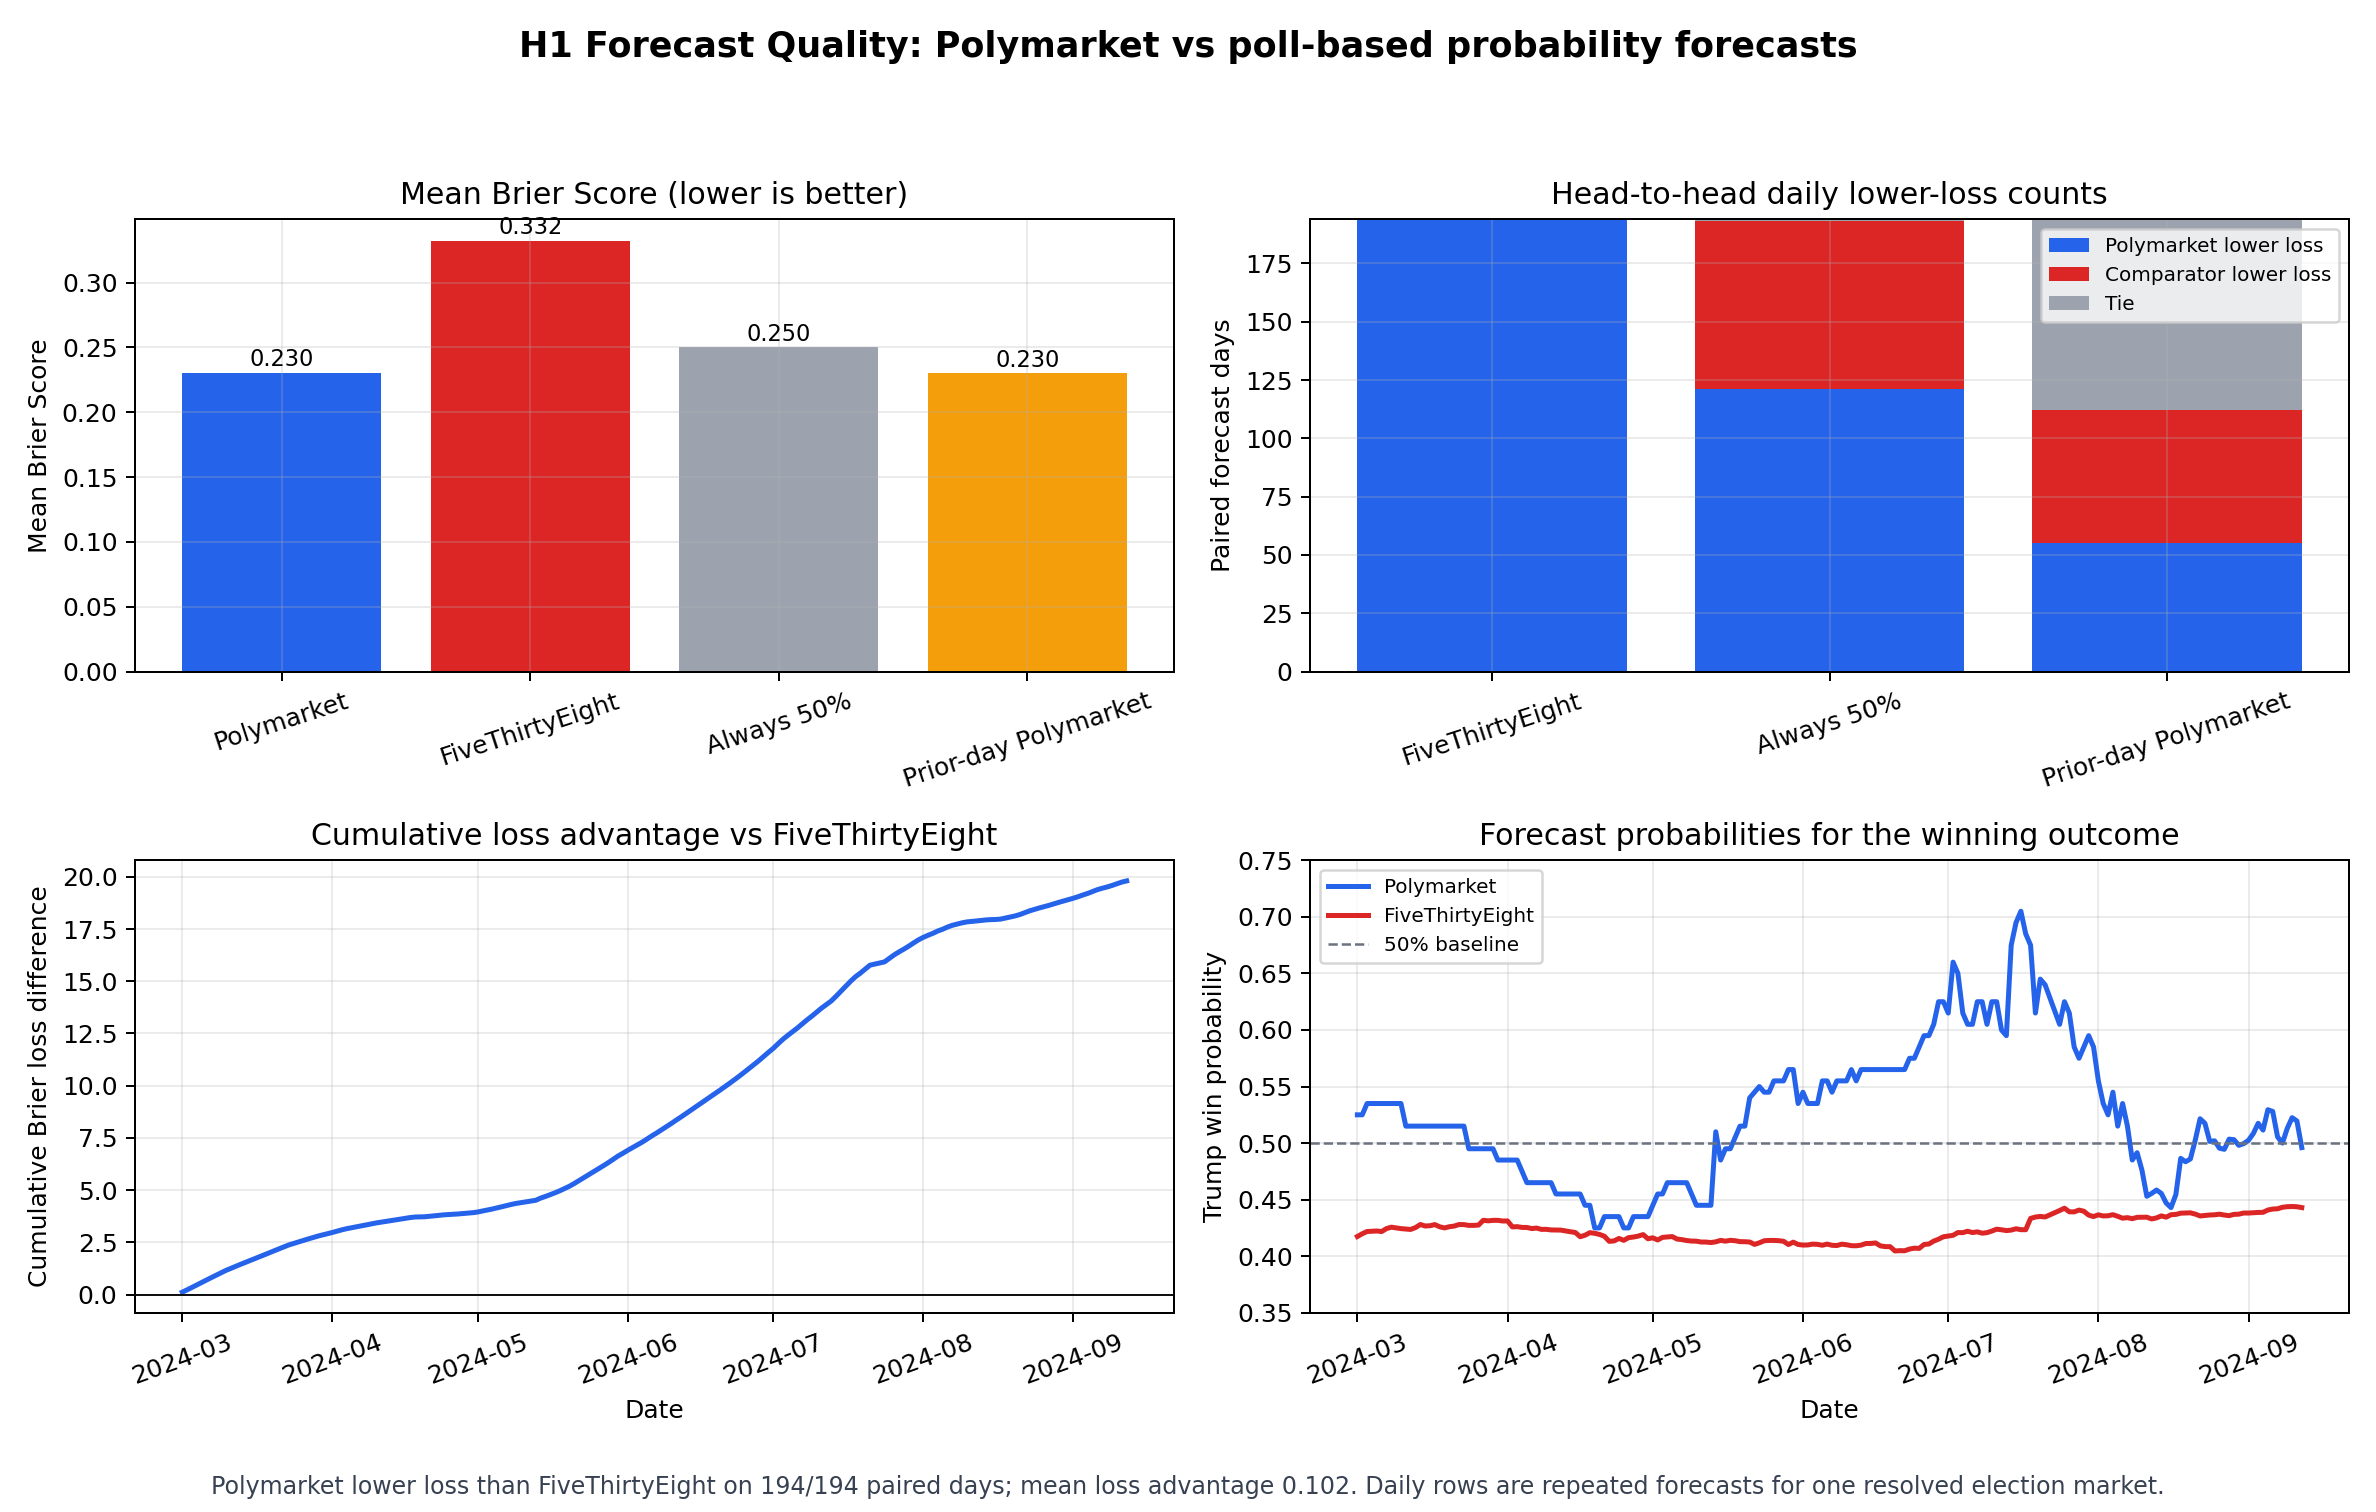
\includegraphics[width=0.82\textwidth]{h1_forecast_quality.png}
\caption{H1-Prognosequalität: Brier-Verlust von Polymarket gegen traditionelle
Vergleichsquellen, Head-to-Head-Zählung und kumulativer Verlustvorteil. Quelle:
\texttt{data/results/h1\_forecast\_quality.png}.}
\label{fig:h1quality}
\end{figure}

\paragraph{Lesart der Abbildung.}
Die Abbildung übersetzt den Befund in drei Ansichten: den paarweisen Brier-Verlust
von Polymarket gegen die Vergleichsquellen, die Head-to-Head-Zählung der Vergleiche
mit tieferem Verlust und den kumulierten Verlustvorteil über die Zeit. Die
Head-to-Head-Zählung macht sichtbar, dass der Vorteil breit über die 285 Zeilen
verteilt ist und nicht von wenigen Ausreissern stammt, während der kumulierte
Verlauf zeigt, ob er anhält. Weil der Brier-Score eine strikt-proper Scoring Rule
ist \citep{lit_gneiting_2007}, lässt sich der tiefere Verlust als bessere, ehrlich
kalibrierte Wahrscheinlichkeit und nicht als blosses Skalenartefakt lesen. Das
Muster reiht sich in die Markt-vs-Umfrage-Evidenz etablierter Prognosemärkte ein
\citep{lit_berg_2008}, bleibt aber auf den definierten Scope beschränkt.

\paragraph{Breite Behauptung nicht bewiesen.}
Über die gesamte Evidenz bleibt die allgemeine Überlegenheit ungedeckt. Von
neun Aggregat-Vergleichszeilen stützen sieben Polymarket im mittleren
Brier-Verlust, aber nur drei nach Fallmehrheit, und keine einzige beweist die
breite Mehr-Fälle-Behauptung. Fünf Audit-Zeilen widersprechen der starken
Aussage. Das volle State-Date-Panel ist ein Gegenbeispiel: dort haben die
poll-abgeleiteten Wahrscheinlichkeiten in 1360 von 1720 Zeilen den niedrigeren
Verlust. Tabelle~\ref{tab:t2} und Abbildung~\ref{fig:h1poll} halten gestützten
Scope und Gegenbeispiele nebeneinander.

\begin{table}[ht]
\centering
\caption{H1 --- Prognosequalität und Poll-Vergleich (T2)}
\label{tab:t2}
\small
\begin{tabular}{@{}lll@{}}
\toprule
Vergleichsscope & Polymarket-Stützung & Kennzahl \\
\midrule
$\leq$90 Tage, geringe/mittlere Poll-Distanz & ja (begrenzt) & 262/285 Zeilen (91.9\%), 9/9 States, $p=0.0020$ \\
Volles State-Date-Panel & nein (Gegenbeispiel) & poll-abgeleitet 1360/1720 Zeilen niedriger \\
Breite Mehr-Fälle-Behauptung & nicht bewiesen & 0/9 Broad-Zeilen, 5 Audit-Zeilen dagegen \\
\bottomrule
\end{tabular}
\end{table}

\begin{figure}[ht]
\centering
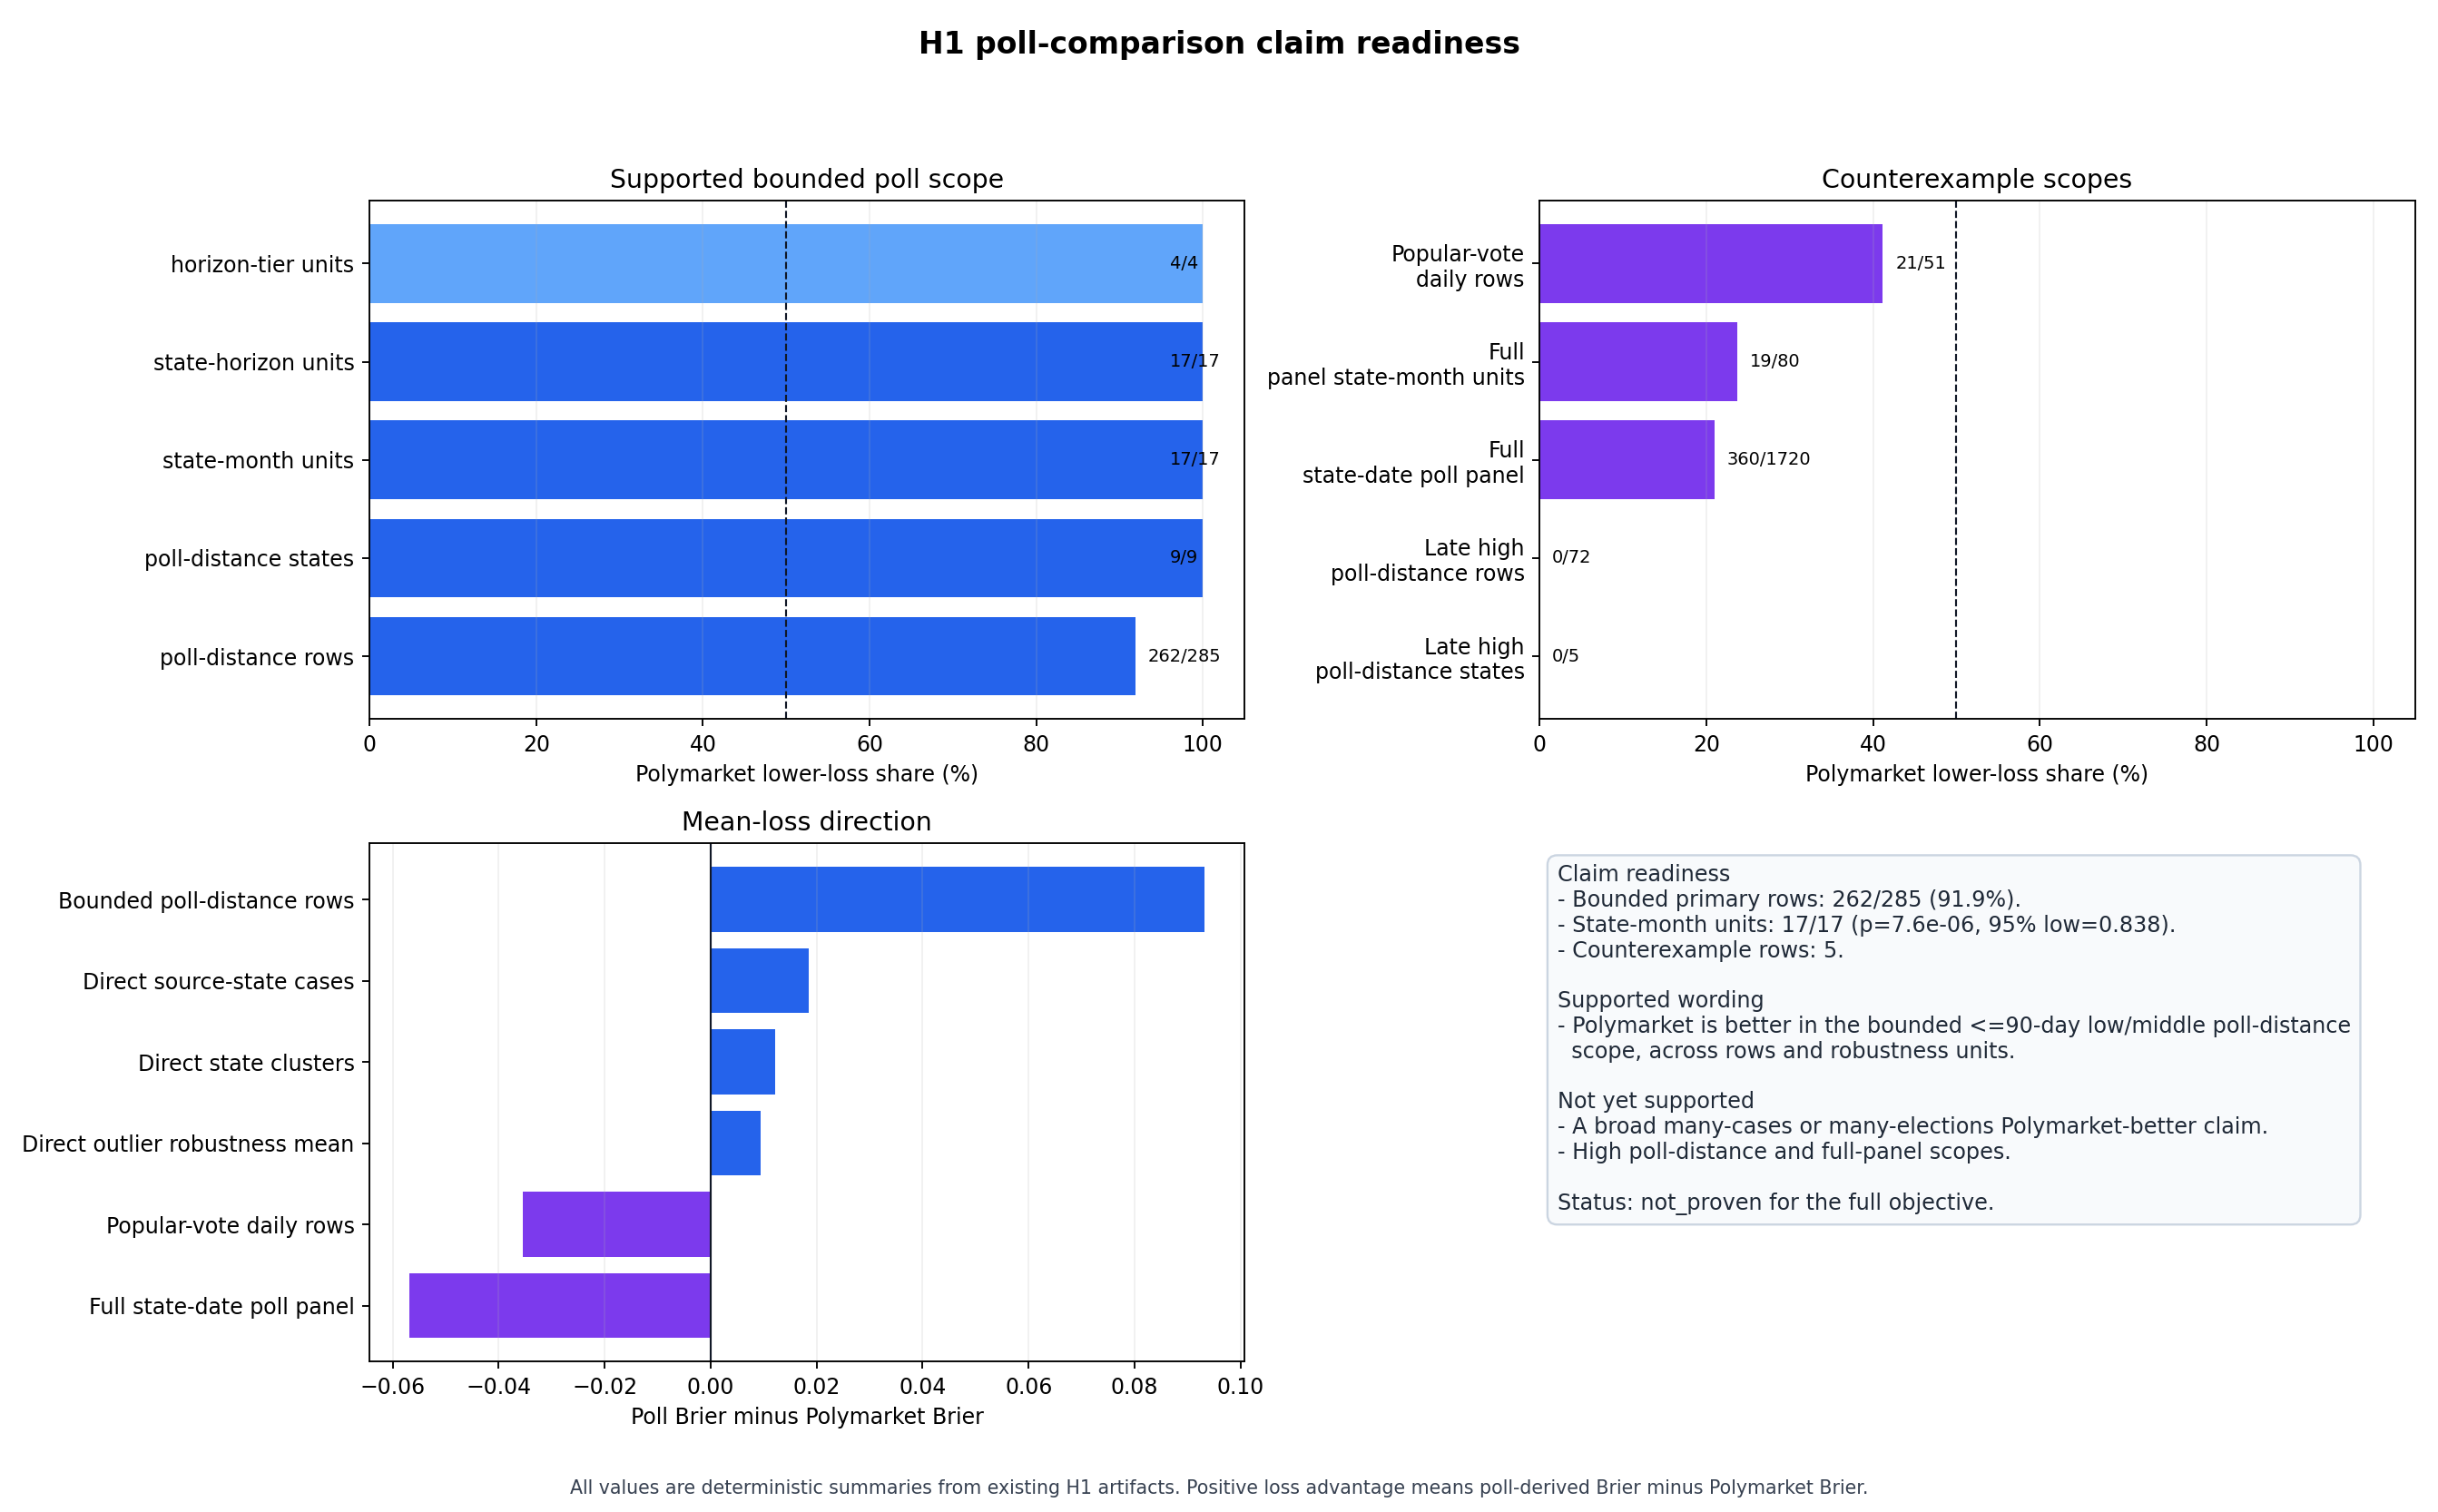
\includegraphics[width=0.82\textwidth]{h1_poll_claim_readiness.png}
\caption{Claim-Readiness des H1-Poll-Vergleichs: gestützter Scope gegen
Gegenbeispiel-Scopes. Quelle: \texttt{data/results/h1\_poll\_claim\_readiness.png}.}
\label{fig:h1poll}
\end{figure}

\paragraph{Lesart der Abbildung.}
Abbildung~\ref{fig:h1poll} stellt den gestützten Scope den Gegenbeispiel-Scopes
gegenüber und macht damit die Kernbotschaft von H1 sichtbar: Der Polymarket-Vorteil
ist real, aber an Bedingungen gebunden (kurzer Horizont, geringe Poll-Distanz). Im
vollen Panel kehrt sich das Bild um. Die Abbildung dient so als
Claim-Readiness-Prüfung, die die belegbare enge Aussage von der nicht belegbaren
breiten Behauptung trennt. Diese Scope-Abhängigkeit deckt sich mit der gemischten,
plattformübergreifenden Evidenz für 2024, in der Marktüberlegenheit nicht
durchgängig auftrat \citep{lit_poly24_accuracy}.

\paragraph{Kalibrierung.}
Die Kalibrierungsdiagnostik in Abbildung~\ref{fig:h1calib} ergänzt den reinen
Verlustvergleich. Über 192 aufgelöste Forecast-Fälle aus sieben Quellen ergeben
sich fünf paarweise Vergleiche. Alle fünf stützen Polymarket im mittleren
Brier-Verlust, aber nur zwei nach Fallmehrheit. Das bestätigt das zweigeteilte
Bild: Polymarket ist im Mittel besser kalibriert, ohne in jedem Einzelfall zu
führen.

\begin{figure}[ht]
\centering

\includegraphics[width=0.82\textwidth]{h1_calibration_diagnostic.png}
\caption{H1-Kalibrierungsdiagnostik über aufgelöste Forecast-Fälle (Scorecard und
Reliabilitätspunkte für Quellen mit mindestens 30 Fällen). Quelle:
\texttt{data/results/h1\_calibration\_diagnostic.png}.}
\label{fig:h1calib}
\end{figure}

\paragraph{Lesart der Abbildung.}
Die Kalibrierungsabbildung kombiniert eine Scorecard der paarweisen Vergleiche mit
Reliabilitätspunkten für Quellen mit mindestens 30 Fällen, dargestellt mit gleichem
Achsenmassstab, sodass die 45-Grad-Diagonale die perfekte Kalibrierung markiert.
Punkte nahe dieser Diagonale stehen für gute Kalibrierung, also prognostizierte
nahe beobachteter Häufigkeit. Dass alle fünf paarweisen Vergleiche Polymarket im
mittleren Brier stützen, aber nur zwei nach Fallmehrheit, zeigt einen im Mittel
besser kalibrierten, jedoch nicht durchgängig führenden Forecast. Das passt zur
Mahnung, einen Marktpreis nicht unbesehen mit einer Wahrscheinlichkeit
gleichzusetzen \citep{lit_manski_2006}.

\paragraph{Limitation.}
Die Evidenz besteht aus wiederholten Tageszeilen innerhalb eines einzelnen
Wahlkontexts und ersetzt keine unabhängige Mehr-Wahlen-Stichprobe. Aus H1
folgt kein Beweis höherer Reaktionsgeschwindigkeit, keine universelle
Marktüberlegenheit und keine kausale Erklärung. Die finale Zitation der
Methodenquellen steht bis zum Abschluss des manuellen Quellen-Reviews aus.

% Status: result_ready_with_limits. Bounded-draft-ready.
% Evidence: interpretation_h2_daily_response
% Artefakte: h2_event_window_summary.csv; events_timeline_seed.csv
\chapter{H2: Ereignisfenster}
\label{ch:h2}

H2 prüft, ob sich Polymarket-Wahrscheinlichkeiten um sieben vorab kuratierte
öffentliche Ereignisse in plausibler Richtung und innerhalb fester Tagesfenster
bewegen \citep{lit_eventstudy_001,lit_emh_001}. Die Ereignisse wurden vor der
Analyse mit Zeitstempel und erwarteter Richtung fixiert.

\paragraph{Sichtbare Tagesreaktion.}
Die stärkste Primärfenster-Bewegung (0--1 Tag) zeigt das Attentat auf Trump am
13.~Juli 2024 mit einer abnormalen Veränderung von $+7.2$ Prozentpunkten zugunsten
von Trump. Die gerichtet erwarteten Ereignisse bewegen sich konsistent: die
Verurteilung im Schweigegeld-Prozess ($-4.1$ pp) und Bidens Rückzug zugunsten
von Harris ($-1.7$ pp für Trump) gehen in die erwartete Richtung. Die übrigen,
als neutral kuratierten Ereignisse zeigen kleinere Bewegungen. Insgesamt
reagieren die Polymarket-Wahrscheinlichkeiten auf Tagesebene plausibel auf die
kuratierten Ereignisse.

\begin{table}[ht]
\centering
\caption{H2 --- Abnormale Veränderung im Primärfenster (0--1 Tag) (T3)}
\label{tab:t3}
\small
\begin{tabular}{@{}llr@{}}
\toprule
Ereignis (2024) & erwartete Richtung & abn. Veränderung (pp) \\
\midrule
Trump-Verurteilung (30.05.) & Trump runter & $-4.1$ \\
Biden--Trump-Debatte (28.06.) & neutral & $+2.5$ \\
Attentat auf Trump (13.07.) & Trump rauf & $+7.2$ \\
Vance als VP (15.07.) & neutral & $+3.5$ \\
Biden-Rückzug (21.07.) & Harris rauf & $-1.7$ \\
Walz als VP (06.08.) & neutral & $+1.3$ \\
Harris--Trump-Debatte (11.09.) & neutral & $-2.9$ \\
\bottomrule
\end{tabular}
\end{table}

\begin{figure}[ht]
\centering
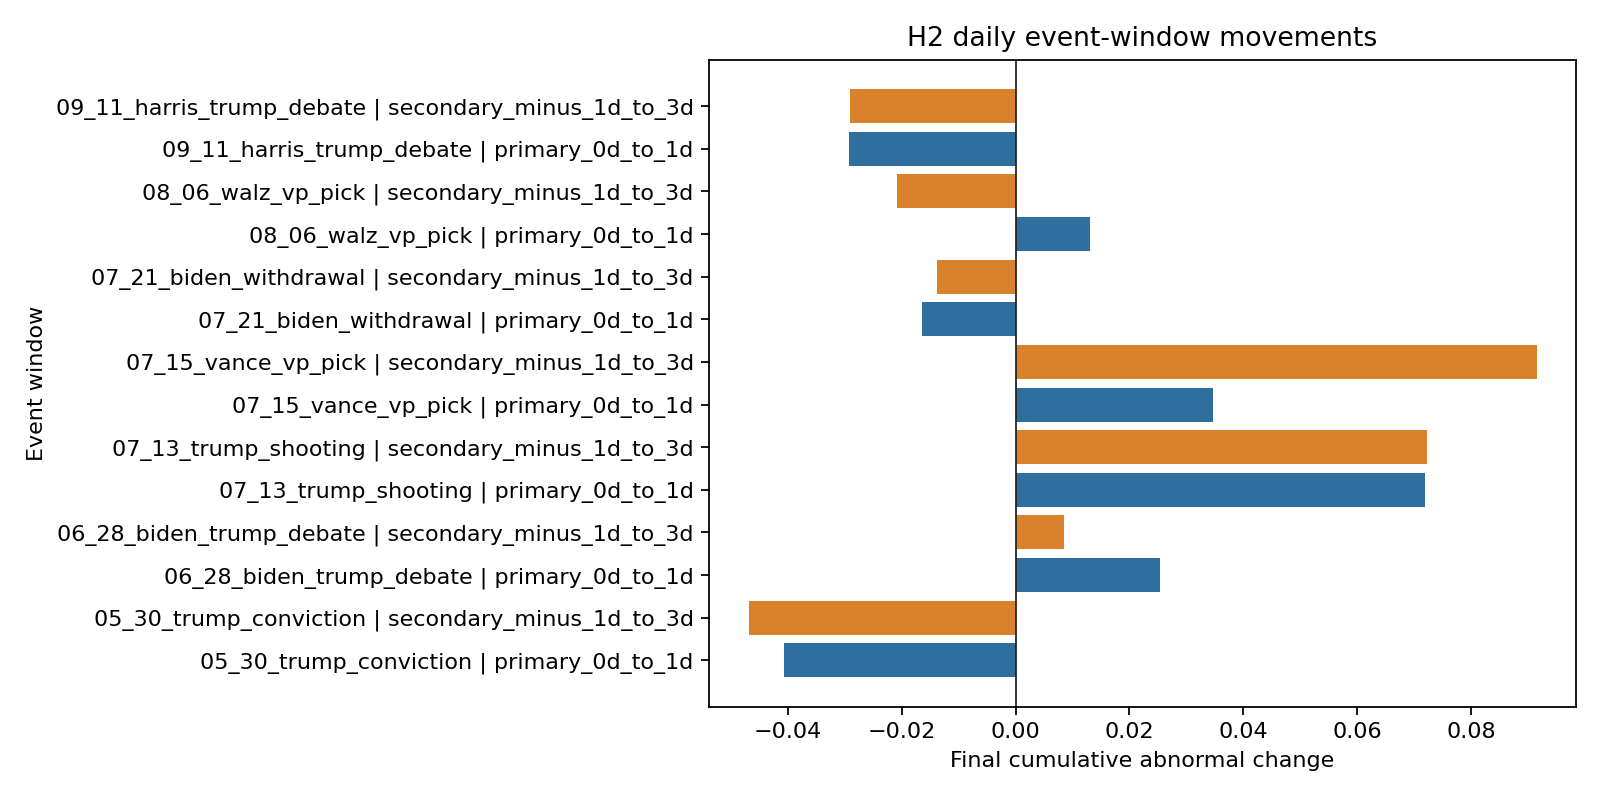
\includegraphics[width=0.85\textwidth]{thesis_h2_event_window_car.png}
\caption{Tägliche Ereignisfenster-Bewegungen (F2). Quelle:
\texttt{data/results/thesis\_h2\_event\_window\_car.png}.}
\label{fig:f2}
\end{figure}

\paragraph{Limitation.}
Die Analyse beruht auf Tagespreisen und kann keine Intraday-Reaktionszeit
identifizieren, H2 stützt damit eine Aussage über tägliche Reaktionsmuster,
nicht über sofortige Marktreaktion. Da die Ereignisse vorab fixiert wurden,
besteht keine nachträgliche Auswahl nach sichtbaren Preisbewegungen.

% Status: result_ready_with_limits. Bounded-draft-ready.
\chapter{H3: Wallet-Timing}
\label{ch:h3}

H3 untersucht, ob dataset-relative Wallet-Tiers zeitliche Aktivitätsmuster vor
oder um Polymarket-Preisbewegungen zeigen. Die Tiers werden aus den beobachteten
kumulierten Betragsperzentilen der Wallet-Verteilung abgeleitet, nicht über eine
willkürliche USD-Schwelle \citep{zotero_poly_001,zotero_poly_007}. Die
Timing-Diagnostik nutzt Lead-Lag-Korrelationen und Granger-Tests
\citep{lit_granger_001}.

\paragraph{Wallet-Tiers.}
Abbildung~\ref{fig:h3tiers} zeigt die verteilungsbasierten Tiers und ihre
Besetzung. Das oberste Tier umfasst das oberste eine Prozent der Wallets
(32 Adressen im beobachteten, BUY-seitigen Datensatz). Die Tiers sind damit
relativ zum Datensatz definiert und tragen keine externe Schwelle.

\begin{figure}[ht]
\centering
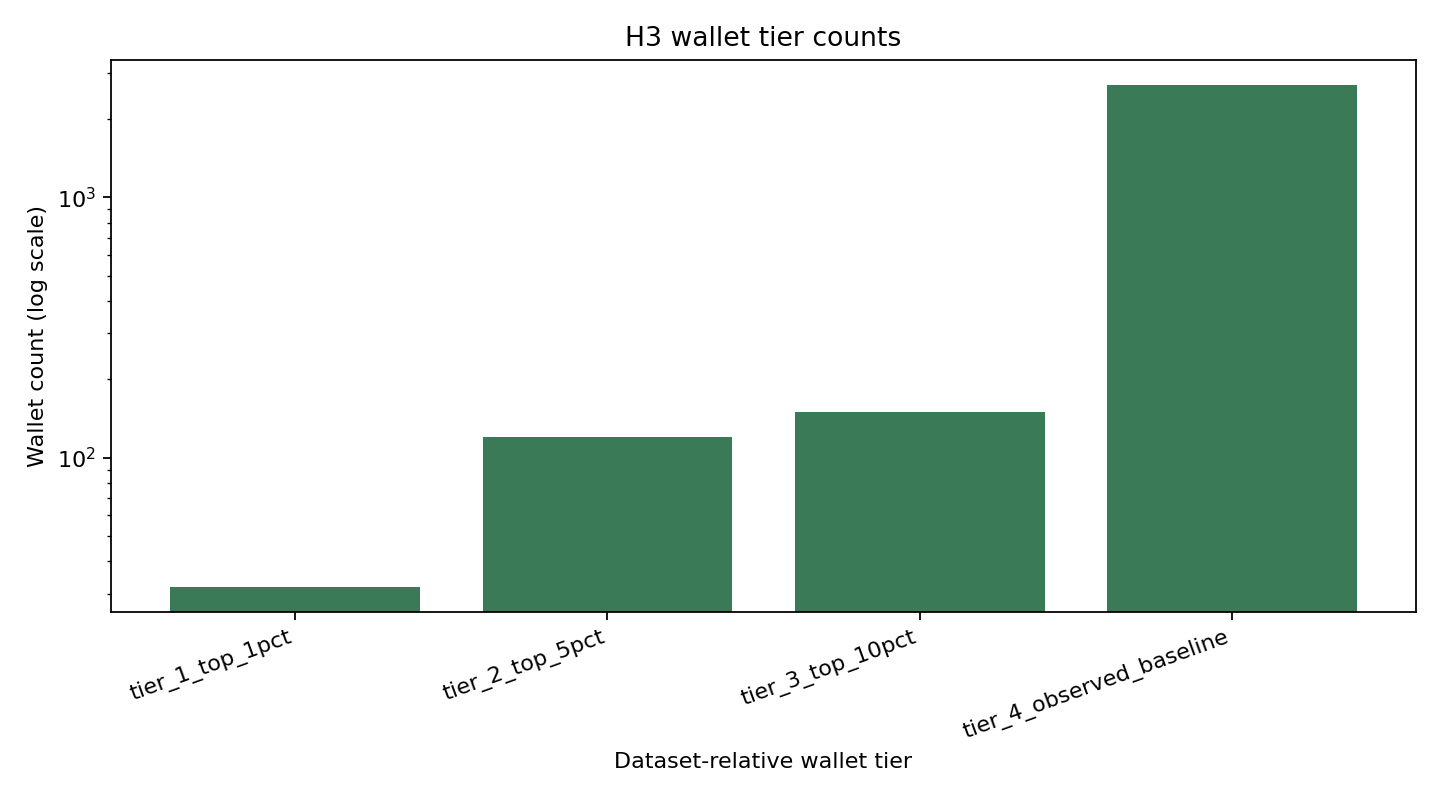
\includegraphics[width=0.78\textwidth]{thesis_h3_wallet_tier_counts.png}
\caption{Dataset-relative Wallet-Tiers und ihre Besetzung. Quelle:
\texttt{data/results/thesis\_h3\_wallet\_tier\_counts.png}.}
\label{fig:h3tiers}
\end{figure}

\paragraph{Klarstes Muster im obersten Tier.}
Das oberste Tier zeigt die deutlichste deterministische Timing-Struktur: eine
Lag-1-Korrelation von $0.186$ zwischen Tier-Aktivität und nachfolgenden
Preisänderungen und einen minimalen Granger-$p$-Wert von $0.0012$ über 1216
ausgerichtete Tageszeilen (Abbildung~\ref{fig:h3granger}). Das ist ein
prädiktives Timing-Signal unter den getesteten Modellannahmen, kein Nachweis
von Kausalität oder privater Information \citep{zotero_poly_005}.

\begin{figure}[ht]
\centering
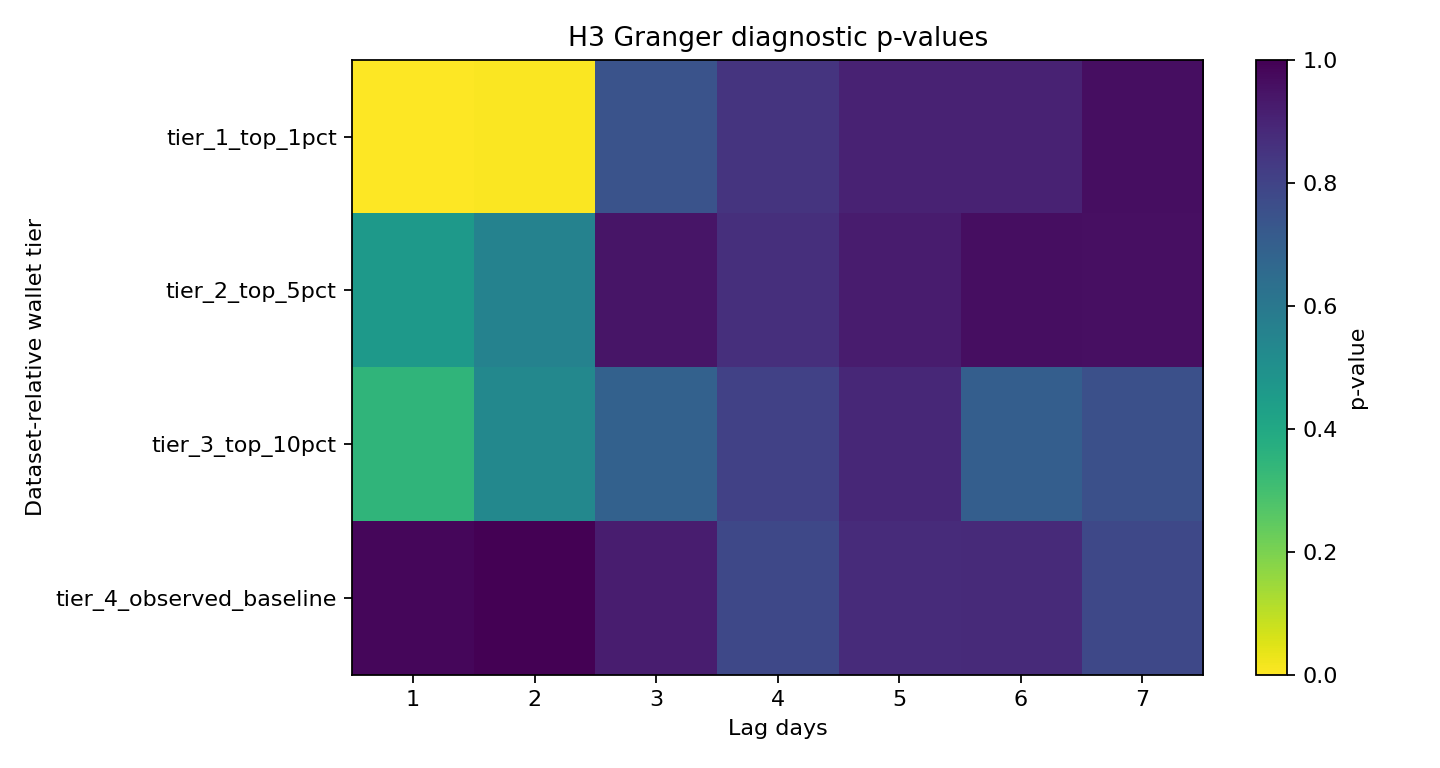
\includegraphics[width=0.78\textwidth]{thesis_h3_granger_pvalues.png}
\caption{Granger-Diagnostik je Tier (minimale $p$-Werte). Quelle:
\texttt{data/results/thesis\_h3\_granger\_pvalues.png}.}
\label{fig:h3granger}
\end{figure}

\paragraph{Deskriptives Lead-Time-Profil.}
Abbildung~\ref{fig:h3lead} stellt die Lead-Time der Tier-Aktivität relativ zu
ausgewählten Bewegungen dar. Das Profil ist rein deskriptiv und beschreibt, wie
sich beobachtete Aktivität zeitlich um Preisänderungen verteilt, ohne eine
Wirkungsrichtung zu behaupten.

\begin{figure}[ht]
\centering
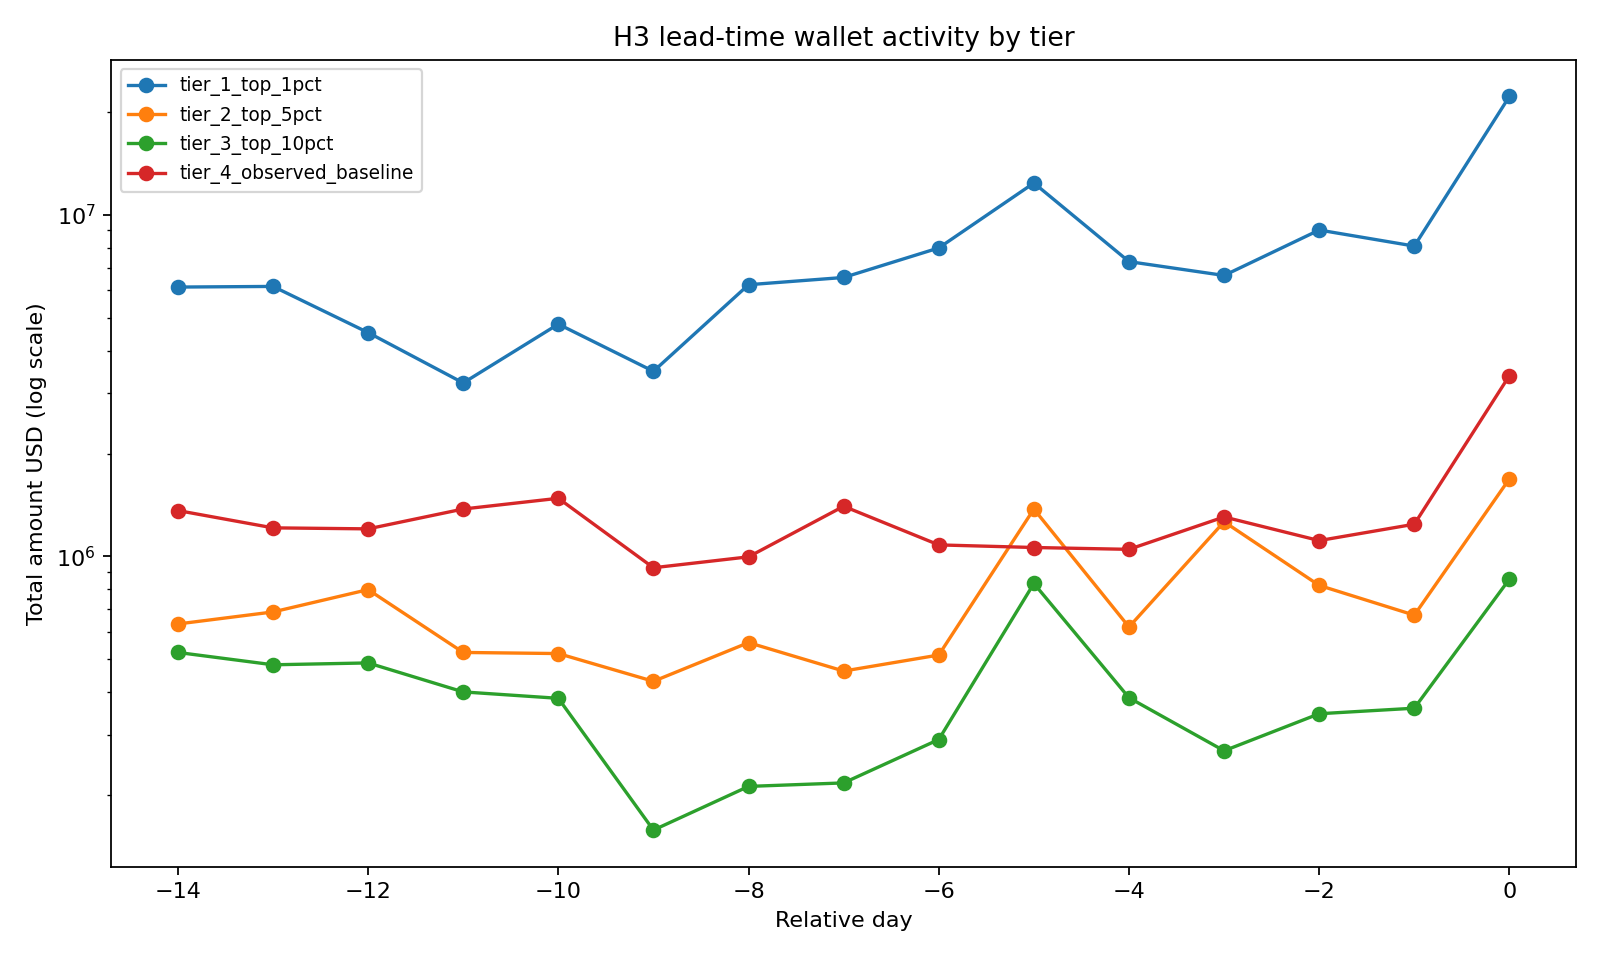
\includegraphics[width=0.78\textwidth]{thesis_h3_lead_time_amount.png}
\caption{Deskriptives Lead-Time-Profil der Tier-Aktivität. Quelle:
\texttt{data/results/thesis\_h3\_lead\_time\_amount.png}.}
\label{fig:h3lead}
\end{figure}

\begin{table}[ht]
\centering
\caption{H3 --- Wallet-Tier-Timing-Diagnostik (T4)}
\label{tab:t4}
\small
\begin{tabular}{@{}lrrr@{}}
\toprule
Tier & Lag-1-Korrelation & Granger-$p$ (min) & ausgerichtete Zeilen \\
\midrule
Oberstes 1\%-Tier & $0.186$ & $0.0012$ & 1216 \\
\bottomrule
\end{tabular}
\end{table}

\section{Ereignis-Wallet-Anomalien als deskriptive Diagnostik}
\label{sec:anomalie}
Auf derselben Datenbasis prüft eine deterministische Anomalie-Diagnostik, ob sich
um die kuratierten Ereignisse auffällige Aktivitäts-, Bewegungs- oder
Konzentrationsmuster zeigen. Eine Tagesbeobachtung gilt als auffällig, wenn ihr
robuster $z$-Wert mindestens $2.0$ erreicht oder ihr Perzentilrang mindestens
$0.95$ beträgt, gemessen gegen ein Basisfenster von 30 bis 8 Tagen vor dem
Ereignis und ein Ereignisfenster von einem Tag davor bis drei Tage danach. Die
Diagnostik betrachtet vier Familien: aktive Wallets je Tier, absolute
Marktbewegung, Top-Tier-Konzentration und Tier-Betragssumme.

Als Beispiel zeigt die Verurteilung im Schweigegeld-Prozess vom 30.~Mai 2024 im
Basis-Tier eine deutliche Aktiv-Wallet-Auffälligkeit ($z = 3.5$, Perzentilrang
$1.0$, zwei auffällige Tage) sowie eine auffällige Marktbewegung
(Perzentilrang $0.96$, ein Tag). Abbildung~\ref{fig:h3anom} fasst über alle
sieben Ereignisse zusammen, welche Familien an welchen Ereignissen auffällige
Tage aufweisen.

\begin{figure}[ht]
\centering
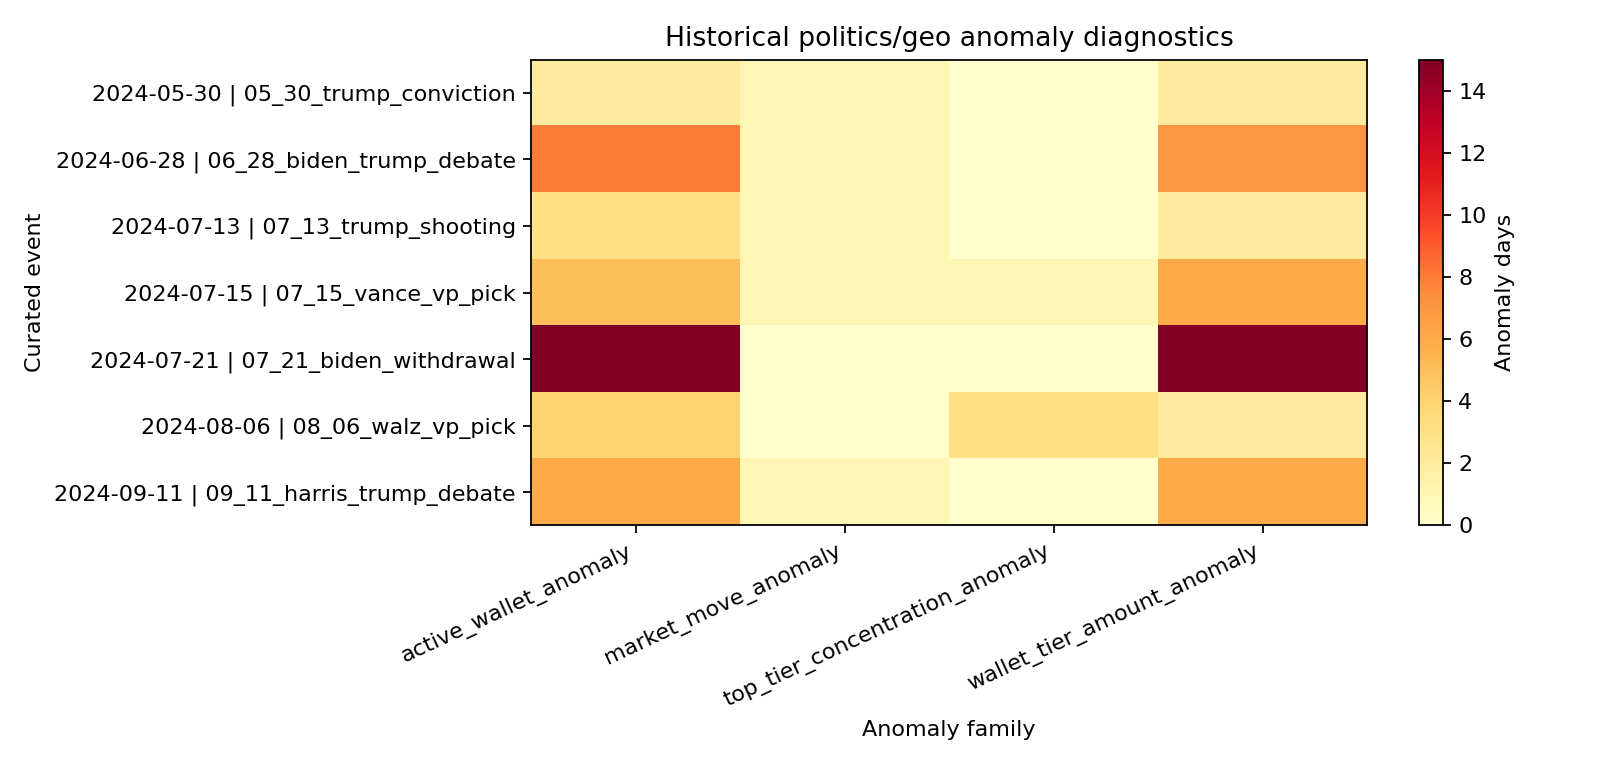
\includegraphics[width=0.82\textwidth]{thesis_h3_event_wallet_anomalies.png}
\caption{Ereignis-Wallet-Anomalien je Ereignis und Anomalie-Familie
(deskriptiv). Quelle: \texttt{data/results/thesis\_h3\_event\_wallet\_anomalies.png}.}
\label{fig:h3anom}
\end{figure}

\paragraph{Was die Diagnostik nicht ist.}
Die Diagnostik arbeitet ausschliesslich mit aggregierten Tier-Zählungen und gibt
keine Wallet-Adressen aus. Sie ist als historische, deskriptive
Auffälligkeits-Diagnostik zu lesen und liefert Prüf-Hinweise, kein Beweis von
privater Information, Insiderhandel, Fehlverhalten, Kausalität oder
Profitabilität. Die spätere Review-Schicht, die solche Hinweise einordnet, wird
in Kapitel~\ref{ch:erweiterungen} beschrieben.

\paragraph{Limitation.}
Die Wallet-Daten enthalten nur Kauftransaktionen und sind quellseitig gefiltert,
die Ausrichtung erfolgt auf Tagesebene, und über mehrere Tiers und Lags hinweg
besteht ein Multiple-Testing-Problem. Die Granger- und Anomalie-Ausgaben sind
deshalb als prädiktive Timing- und Auffälligkeits-Diagnostik zu lesen, nicht als
Beweis von Kausalität, privater Information oder Profitabilität.

\section{Signaturen informierten Handels und ein Verdachts-Profil}
\label{sec:verdacht}
Forschung und Praxis nennen wiederkehrende Signaturen informierten oder
Insider-Handels: frische Wallets mit wenigen Lebenstransaktionen, die grosse
Positionen eingehen, ungewöhnliche Positionsgrösse vor noch nicht angekündigten
Ausgängen, abnormale Handelsgrösse und Volumen, hohe Konzentration und
einseitiger Fluss sowie Aktivität, die sich gegen die Marktauflösung verdichtet.
Akademisch zeigt \citet{zotero_delvecchio_001} für Kalshi-Märkte, dass
informierter Handel real und über eine Abnormal-Trade-Size-Kennzahl detektierbar
ist und sich gegen die Auflösung verstärkt, im Einklang mit dem Insider-Modell
von \citet{lit_kyle_001}. Praktisch setzt Polymarket eine On-Chain-Überwachung
ein, die unter anderem ungewöhnliche Positionsgrösse vor Ergebnissen und
auffällige Wallets flaggt \citep{news_polymarket_integrity_001}, gestützt auf
forensische Heuristiken wie Funding-Quellen und Wallet-Clustering
\citep{news_chainalysis_forensics_001}. Konzeptionell rahmt
\citet{zotero_poly_005} Insiderhandel in Prognosemärkten.

\paragraph{Profil aus dem getesteten Signatur-Modul.}
Dieselben Signaturen werden in einem deterministischen, getesteten Modul (\texttt{informed\_trading\_signature}) auf den BUY-seitigen Whale-Datensatz
(ab 10\,000 USD) anwenden. In den sieben Ereignisfenstern dominieren neu
erscheinende Wallets. Im Median traten 54\% der aktiven Wallets erst um das
Ereignis herum erstmals auf (Spanne 48--69\%), bei einer Top-1-Konzentration von
im Median 64\% (54--81\%) und gegenüber der Vorperiode erhöhter
Aktivität und erhöhtem Volumen (Abbildung~\ref{fig:h3profile}). Das Modul fasst die Einzel-Signaturen perzentil-normalisiert zu einem \texttt{suspicion\_score} zusammen (Spanne 0.10--0.81, Median 0.55). Dieses Muster
deckt sich mit der Literatur-Signatur aus frischen Wallets, grosser
Positionsgrösse und Konzentration.

\begin{figure}[ht]
\centering
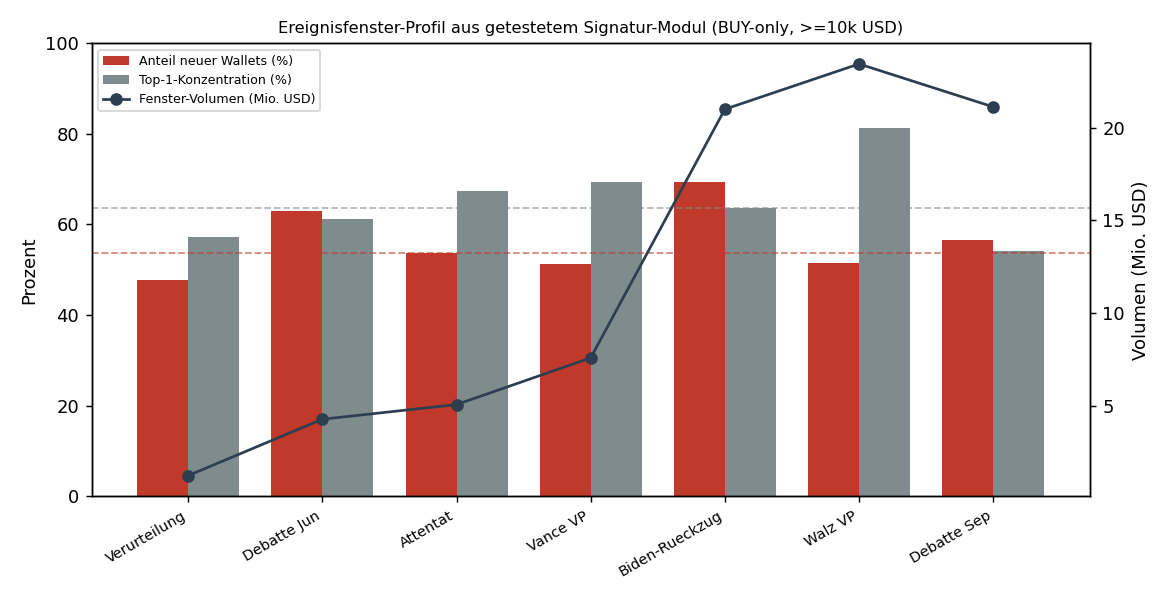
\includegraphics[width=0.86\textwidth]{h3_informed_trading_profile.png}
\caption{Ereignisfenster-Profil aus dem getesteten Signatur-Modul: Anteil neuer Wallets,
Top-1-Konzentration und Fenster-Volumen je Ereignis (BUY-only, ab 10\,000 USD).
Quelle: \texttt{data/results/h3\_informed\_trading\_signature.csv}.}
\label{fig:h3profile}
\end{figure}

\paragraph{Verdachts-Profil als Hypothese.}
Daraus folgt ein Verdachts-Profil, das als Hypothese und Prüf-Filter dient. Ein
Ereignisfenster ist prüfwürdig, wenn mehrere Signaturen gemeinsam auftreten --
ein hoher Anteil neuer Wallets, hohe Konzentration, abnormale Aktiv-Wallet- und
Volumen-Werte aus Abschnitt~\ref{sec:anomalie} sowie ein Vorlauf der
Tier-Aktivität vor der Preisbewegung aus der Lead-Lag- und Granger-Diagnostik.
Genau diese Kombination speist die Review-Queue in
Kapitel~\ref{ch:erweiterungen}.

\paragraph{Was das Profil nicht beweist.}
Ein hoher Anteil neuer Wallets ist kein Insider-Nachweis. Aufmerksamkeitsstarke
Ereignisse ziehen allgemein neue Teilnehmer an, frische Adressen entstehen auch
aus Datenschutz- oder Komfortgründen, und der Datensatz ist BUY-only und ab
10\,000 USD gefiltert, was den Anteil neuer Wallets mechanisch erhöht. Zudem
zeigen \citet{zotero_poly_001} für die Oktober-Episode 2024, dass Kapital auf
beide Marktseiten floss, vereinbar mit heterogenen Erwartungen statt
Manipulation. Das Profil bleibt damit eine Verdachts-Hypothese und ein
Prüf-Filter, kein Nachweis privater Information.

\paragraph{Was die Diagnostik härten würde.}
Zur Härtung fehlen deterministische, getestete Merkmale: die Funding-Quelle der
Wallets (zentrale Börse oder Mixer), Wallet-Lebensdauer und Transaktionszahl,
einseitiger Fluss je Markt, der Vorlauf gegenüber verifizierten
Nachrichten-Zeitstempeln und ein Out-of-Sample-Test gegen die wenigen
dokumentierten Insider-Fälle. Diese Erweiterungen sind als Spezifikation
vermerkt und bleiben an die Audit- und Wallet-Adress-Grenzen gebunden.

% Status: Schlussfolgerung aus der Analyse (4b), ausgeschrieben.
\chapter{Schlussfolgerung aus der Analyse}
\label{ch:schluss}

\section{Synthese der drei Hypothesen}
Die drei Hypothesen ergeben ein konsistentes, aber bewusst begrenztes Bild. H1
zeigt eine bessere Prognosequalität von Polymarket nur in einem klar definierten
Vergleichsscope: In der nationalen Tagesreihe trägt Polymarket den tieferen
mittleren Brier-Verlust (0.230 gegen 0.332 von FiveThirtyEight), und auf
Bundesstaaten-Ebene stützen 262 von 285 Zeilen sowie 9 von 9 Staaten den Vorteil
(exakter Binomialtest, p = 0.0020). Die breite Überlegenheit bleibt jedoch
ungedeckt, und das volle State-Date-Panel ist ein Gegenbeispiel. H2 zeigt plausible
Tagesreaktionen auf die sieben vorab kuratierten Ereignisse, am deutlichsten beim
Attentat auf Trump (+7.2 Prozentpunkte), während die neutral kuratierten Ereignisse
erwartungsgemäss streuen. H3 findet das klarste prädiktive Timing-Muster im
obersten Wallet-Tier (Lag-1-Korrelation 0.186, minimaler Granger-p-Wert 0.0012 über
1216 ausgerichtete Zeilen). Zusammengenommen stützen die Befunde begrenzte,
scope-spezifische Diagnosen informationeller Effizienz, keine universelle Aussage.

\section{Stützende Evidenz ausserhalb der Hypothesen}
Zwei weitere Beobachtungen fügen sich in dieses Bild. Erstens deckt sich der
paper-only Arbitrage-Befund (Kapitel~\ref{ch:loesung}) mit weitgehend effizienten
Märkten: Saubere strukturelle Arbitragen sind selten, die wenigen echten
Cross-Venue-Fälle sind kleine Carry-Trades, und die kaum robust ausnutzbare
Ineffizienz ist selbst ein Effizienz-Indiz. Zweitens lag Polymarket in der
Schweizer Referendums-Fallstudie als binäre Wahrscheinlichkeit auf der richtigen
Seite des Resultats; dies ist jedoch ein transparenter Proxy und ein einzelner,
frischer Datenpunkt ausserhalb der US-Wahl, keine Verallgemeinerung.

\section{Einordnung in die Literatur}
Der begrenzte H1-Vorteil ist mit \citet{zotero_poly_002} vereinbar, die einen
Polymarket-Vorteil besonders in Swing States berichten, zugleich aber zur Vorsicht
bei Verallgemeinerung mahnen. Das Gegenbeispiel im vollen Panel passt zur kritischen
Lesart von \citet{zotero_poly_009}, wonach Prognosemärkte reflexiv statt eine
``Truth Machine'' sind, sowie zur gemischten plattformübergreifenden Evidenz für
2024 \citep{lit_poly24_accuracy}. Die Vorsicht bei H3 deckt sich mit
\citet{zotero_poly_001}, deren Grosskonto-Befund heterogene Erwartungen statt
Manipulation nahelegt, und mit der Insider-Rahmung von \citet{lit_kyle_001} und
\citet{zotero_delvecchio_001}. Insgesamt verarbeiten die Märkte Information
innerhalb von Grenzen gut, vereinbar mit einer halbstrengen Effizienzlesart
\citep{lit_emh_001}, ohne dass Preis und Wahrscheinlichkeit unbesehen
gleichzusetzen wären \citep{lit_manski_2006}.

\section{Folgerung für die Forschungsfrage}
Aus der Analyse folgt, dass Polymarket im untersuchten Kontext Information
nachweisbar gut verarbeitet, aber nur in klar abgegrenzten Fällen messbar besser
als traditionelle Quellen. Diese begrenzte, doch belastbare Diagnose ist der
eigentliche Beitrag: Sie trennt Gestütztes sauber von Nicht-Gestütztem. Genau das
motiviert den folgenden Lösungsteil --- ein Werkzeug, das solche begrenzten,
deterministisch geprüften Hinweise sichtbar und für Menschen prüfbar macht.

% Status: appendix_or_discussion_ready (Monitor/Swiss) + Narrativ-Entscheide.
\chapter{Erweiterungen: Monitor, Schweizer Abstimmung und praktischer Beitrag}
\label{ch:erweiterungen}

Dieses Kapitel ordnet vier Erweiterungen ausserhalb des empirischen Kerns ein.
Sie stützen die Forschungsfrage, ersetzen aber nicht den H1--H3-Beleg.

\section{Schweizer Referendum als begrenzte Fallstudie}
Als aktueller, eigenständiger Vergleich dient die eidgenössische Abstimmung vom
14.~Juni 2026. Beim offiziellen Ja-Anteil von 45.21\% lag die finale Umfrage als
Stimmenanteil näher am Resultat, während Polymarket im lokalen Live-Fenster (Ja
zuletzt 21.5\%) als binäre Ablehnungswahrscheinlichkeit klarer auf der richtigen
Seite lag \citep{zotero_poly_002}. Wichtig: Polymarket-Preise sind
Annahmewahrscheinlichkeiten, Umfragen sind Stimmenanteile. Der Binärvergleich
ist nur ein transparenter Proxy und kein Mispricing-, Effizienz- oder
Tradeability-Beweis (Abbildung~\ref{fig:swiss}).

\begin{figure}[ht]
\centering
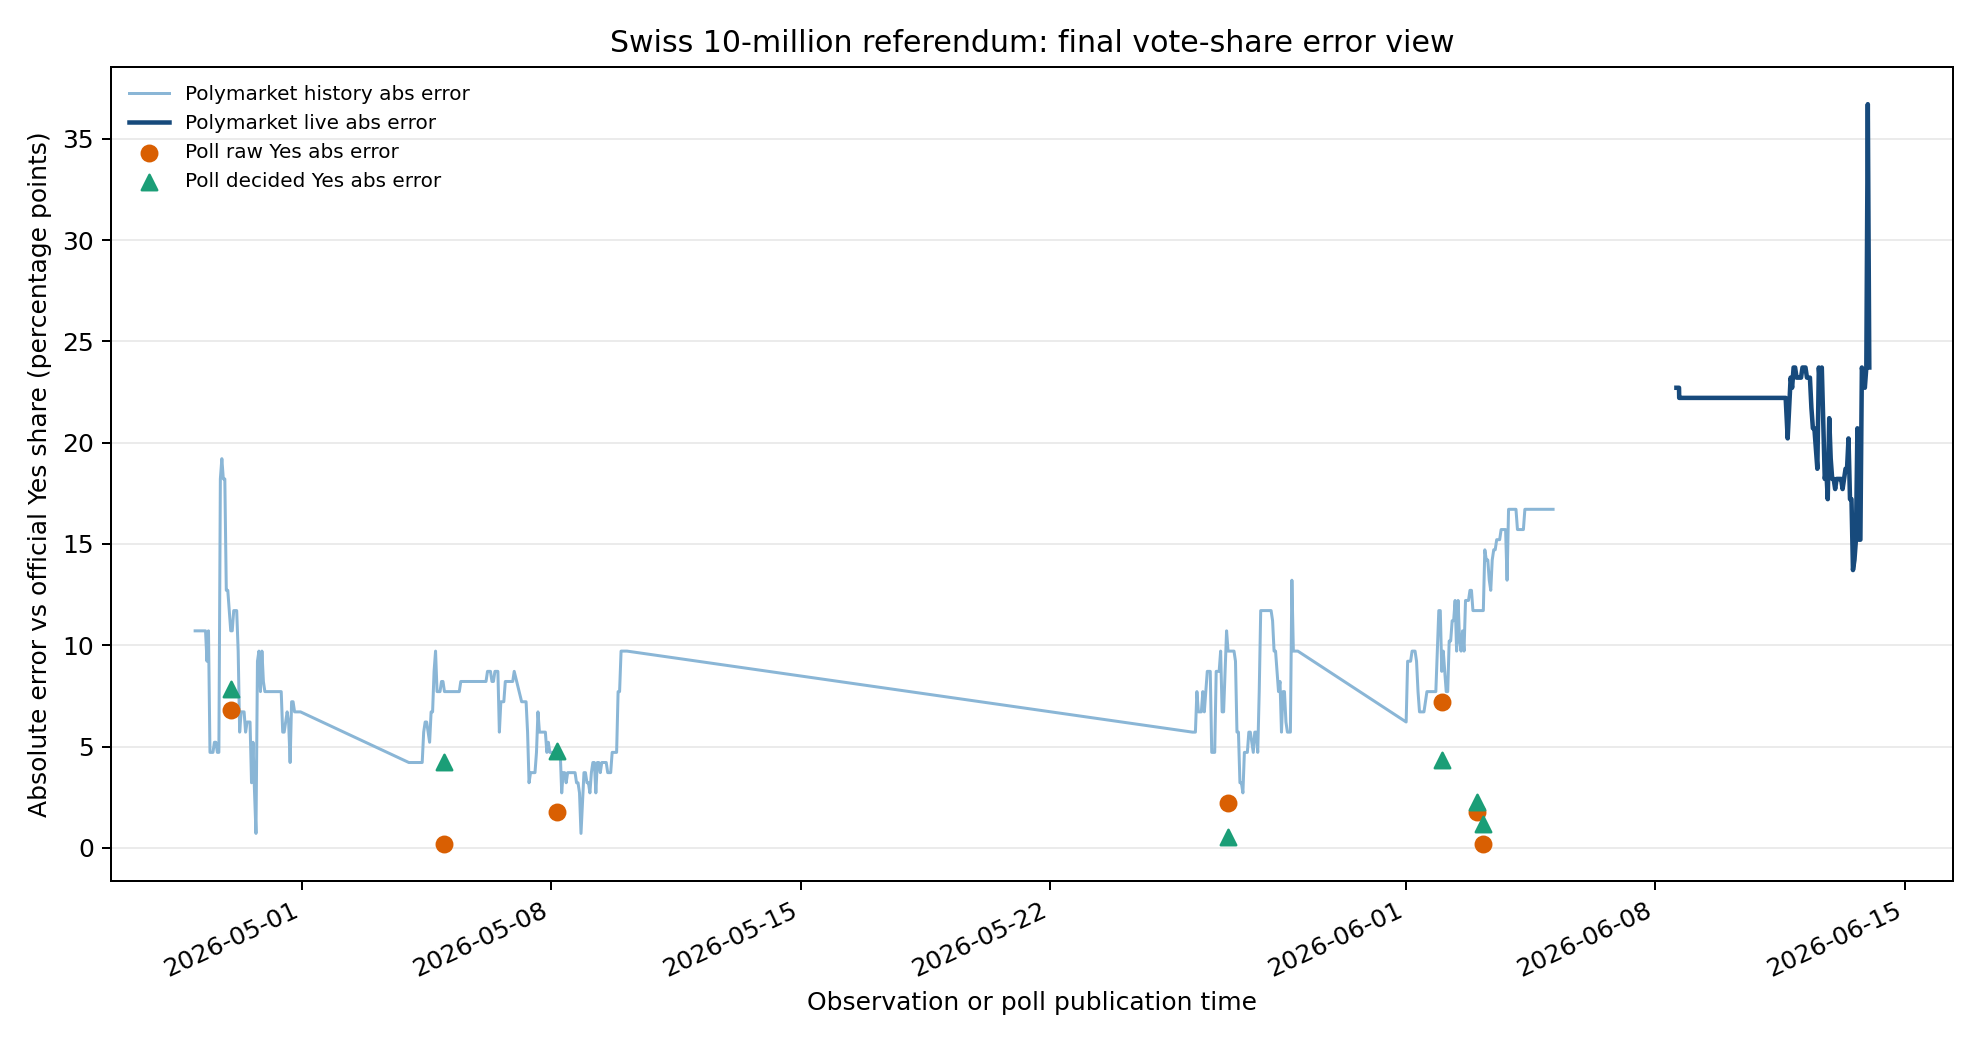
\includegraphics[width=0.82\textwidth]{swiss_referendum_10mio_final_case_study.png}
\caption{Schweizer Referendum 14.~Juni 2026: offizielles Resultat gegen
Polymarket-Preise und Umfrage-Proxy (begrenzte Post-Resultat-Fallstudie).
Quelle: \texttt{data/results/swiss\_referendum\_10mio\_final\_case\_study.png}.}
\label{fig:swiss}
\end{figure}

\section{Anomalie-Review-Queue als Prüf-Workflow}
Die deterministische Anomalie-Diagnostik aus Abschnitt~\ref{sec:anomalie} liefert
Hinweise, die eine nachgelagerte Review-Schicht einordnet. Die aktuelle
Review-Queue enthält drei Fälle: einen mit hoher Priorität, der als
Prüf-Kandidat markiert ist, und zwei mit mittlerer Priorität als Beobachtungs-Hinweis.
Alle drei stehen auf Quellenprüfung ausstehend. Bei der Überlappung mit den
kuratierten Referenzfällen ergeben sich ein Treffer, eine teilweise und eine
fehlende Überlappung.

Diese Queue ist ausdrücklich ein menschlicher Prüf-Workflow über begrenzte,
bereits berechnete Monitor-Artefakte. Die Risiko-Etiketten sind Beobachtungs-Marker,
keine Befunde. Die Queue beweist weder private Information noch Fehlverhalten,
Kausalität, Handelbarkeit, Profitabilität oder künftige Performance.

\section{Politik-/Geo-Monitor als Read-only-Prototyp}
Der Monitor kombiniert Marktbewegung, aggregierte Wallet-Tier-Aktivität,
Konzentration und Ereigniskontext zu deterministischen Prüf-Hinweisen
\citep{zotero_poly_006,zotero_poly_009}. Er bleibt read-only, erzeugt keine
Order- oder Trading-Pfade und liefert Prüf-Hinweise, keine kausale oder
Effizienz-Evidenz. Im Haupttext erscheint er nur als Workflow, Fälle bleiben bis
zur manuellen Prüfung im Anhang.

\section{Agenten-gestützte Pipeline als dokumentierter Vertrag}
Die ursprünglich angestrebte Multiagenten-Pipeline ist hier als bewusst
begrenzter, dokumentierter Vertrag verankert. Künftige Agenten dürfen Hinweise
sichten und einordnen, aber keine Kennzahlen berechnen. Der Vertrag definiert
vier Rollen: einen EventScout, der Ereigniskandidaten sammelt, einen
CaseNarrative, der Fälle aus begrenzten Zusammenfassungen beschreibt, einen
SkepticReviewer, der gegenprüft, und einen Orchestrator, der entscheidet. Eine
spätere, ebenfalls vertraglich begrenzte MCP-Schicht stellt nur lesende Werkzeuge
bereit (Anomalie-Review-Summary, Einzelfall, Artefaktliste, Methodengrenzen), mit
maximal 50 Zeilen je Abfrage, ohne rohes SQL, ohne standardmässige
Wallet-Adress-Ausgabe und mit Pflicht zur Protokollierung jeder LLM-Interaktion.
Beide Verträge sind als nicht implementiert markiert und bleiben Future Work, bis
der deterministische Kern und die Audit-Grenzen vollständig stehen.

\section{Praktischer Beitrag: Monitoring-Werkzeug und Bau-Methodik}
Während der Untersuchung wurde Bedarf an einem praktischen Analyse-Werkzeug für
Prognosemärkte erkennbar. Als Gestaltungsbeitrag wurde daraus ein laufendes,
read-only Webprodukt entwickelt, das die Effizienz-Perspektive der Arbeit
operationalisiert. Die Umsetzung selbst nutzte eine Multiagenten-Orchestrierung
als Entwicklungsmethode, dokumentiert wird diese als Prozessbeitrag. Die Agenten
erzeugten Software, berechneten aber keine thesis-relevanten Kennzahlen. Beide
Punkte sind Sekundärbeiträge und dürfen die Forschungsfrage nicht überlagern.
Umfang und Einordnung sind mit der Betreuung abzustimmen.

% Status: Allgemeine Schlussfolgerung und Einschraenkungen (4b-Struktur).
\chapter{Allgemeine Schlussfolgerung und Einschränkungen}
\label{ch:einschraenkungen}

\section{Gesamtfazit}
Auf die Forschungsfrage antwortet die Arbeit differenziert: Polymarket verarbeitet
Information im untersuchten Kontext nachweisbar gut, aber nur in klar abgegrenzten
Fällen messbar besser als traditionelle Quellen. Die Stärke der Arbeit liegt
weniger in einer einzelnen grossen Behauptung als in der reproduzierbaren,
deterministisch geprüften Trennung von gestützter und nicht gestützter Evidenz
\citep{lit_emh_001}, ergänzt um ein lauffähiges Werkzeug, das diese Trennung
operationalisiert.

\section{Einschränkungen}
Die Evidenz stammt aus einem einzelnen Wahlkontext mit wiederholten Tageszeilen
und erlaubt keine Mehr-Wahlen-Verallgemeinerung. H2 beruht auf Tagesdaten und
identifiziert keine Intraday-Reaktionszeit \citep{lit_eventstudy_001}. Die
H3-Wallet-Daten sind BUY-only und quellseitig gefiltert, die Ausrichtung erfolgt
täglich, und über mehrere Tiers und Lags besteht ein Multiple-Testing-Problem
\citep{lit_granger_001}. Verhaltensverzerrungen und erhöhte Volatilität
\citep{zotero_poly_007} begrenzen die Tragweite zusätzlich. Das Werkzeug bleibt
read-only und liefert Prüf-Hinweise, keine Beweise.

% Status: Naechste Schritte / Ausblick (4b-Struktur). Guarded.
\chapter{Nächste Schritte}
\label{ch:naechste}

Über den empirischen Kern hinaus lässt sich die in Kapitel~\ref{ch:loesung}
vorgestellte Lösung zu einer agentengestützten Assistenzschicht ausbauen, die
künftig die Interpretation begrenzter, bereits berechneter Zusammenfassungen
unterstützt, ohne selbst Kennzahlen zu berechnen.

Künftige Agenten dürfen Entwurfs-, Review- und Quellen-Prüf-Workflows nur aus
begrenzten, bereits deterministisch berechneten Zusammenfassungen unterstützen.
Sie berechnen keine Kennzahlen und greifen nicht ungefiltert auf Rohdaten zu,
jede LLM-Interaktion wird protokolliert. Als Aktivierungs-Gates gelten ein
separates Goal, Tests, bounded inputs (maximal 50 Zeilen je Abfrage) und die
Protokollierung jeder LLM-Interaktion. Weitere Schritte betreffen die Härtung der
Verdachts-Signatur (Funding-Quellen, Wallet-Lebensdauer, Out-of-Sample-Test gegen
dokumentierte Fälle), stets gebunden an die Audit- und Wallet-Adress-Grenzen.


% ====================== Literaturverzeichnis ======================
\bibliographystyle{apacite}
\addcontentsline{toc}{chapter}{Literaturverzeichnis}
\bibliography{references}

\end{document}
